\documentclass{article}

\usepackage{amsmath}
\usepackage{amsthm}
\usepackage{amssymb}
\usepackage{color}
\usepackage{tikz}
\usetikzlibrary{shapes,arrows.meta,backgrounds}
\usepackage{etoolbox}
\usepackage{url} % for urls in bibliography
\usepackage[parfill]{parskip} % no paragraph indents, leave blank line
\usepackage{graphicx}
\usepackage{subcaption}
\usepackage{listings}
\usepackage{xifthen}% provides \isempty test

\graphicspath{ {./drawio/} }

% Need this to keep the space before theorems when using parfill parskip
% https://tex.stackexchange.com/questions/25346/wrong-spacing-before-theorem-environment-amsthm
\begingroup
    \makeatletter
    \@for\theoremstyle:=definition,remark,plain\do{%
        \expandafter\g@addto@macro\csname th@\theoremstyle\endcsname{%
            \addtolength\thm@preskip\parskip
            }%
        }
\endgroup

\DeclareRobustCommand{\rchi}{{\mathpalette\irchi\relax}}
\newcommand{\irchi}[2]{\raisebox{\depth}{$#1\chi$}} % inner command, used by \rchi

\usepackage{mathtools}
\usepackage{bm}
\usepackage{stmaryrd} % for llbracket and rrbracket

\theoremstyle{definition}
\newtheorem{example}{Example}[section]
\newtheorem{defn}{Definition}[section]

\newcommand{\adj}[1]{\llbracket #1 \rrbracket} 
\newcommand{\enf}[1]{[#1]} 

\newcommand{\holds}[3]{#1 %
  \ifthenelse{\isempty{#2}}{}{{:} #2} %
  \ifthenelse{\isempty{#3}}{}{\mapsto #3} %
} 
\newcommand{\alloc}[1]{( #1 )} 
\newcommand{\guar}[2]{( #1 | #2 )} 

\newcommand{\finalizable}[3]{[#1 \mapsto #2]_{#3}}
\newcommand{\transfer}[3]{T_{#1, #2}(#3)}
\newcommand{\claim}[3]{C_{#1, #2}(#3)}


\usepackage{xparse}
% https://tex.stackexchange.com/a/55604

\usepackage{tikz}
\usetikzlibrary{shapes,backgrounds,calc}
\usetikzlibrary{positioning, shapes.geometric}

\makeatletter
\tikzset{fill halves/.style  args={#1,#2}{%
  circle,
  postaction={%
    insert path={
      \pgfextra{% 
        % This entire script assumes that we're working with a circle, making use of the anchors
        % we expect to find on a circle
        % Calculates "insiderad" by looking at the distance from the center to the east anchor
        \pgfpointdiff{\pgfpointanchor{\pgf@node@name}{center}}%
                    {\pgfpointanchor{\pgf@node@name}{east}}%            
        \pgfmathsetmacro\insiderad{\pgf@x}
        % We start at the east anchor of the node and then move in by "pgflinewidth"
        % then we draw an arc from 0 to 180
        \fill[#1] (\pgf@node@name.base) ([xshift=-\pgflinewidth/sqrt(2), yshift=-\pgflinewidth/sqrt(2)]\pgf@node@name.north east) arc
                          (45:225:\insiderad-\pgflinewidth)--cycle;
        \fill[#2] (\pgf@node@name.base) ([xshift=\pgflinewidth/sqrt(2), yshift=\pgflinewidth/sqrt(2)]\pgf@node@name.south west)  arc
                            (225:405:\insiderad-\pgflinewidth)--cycle;
        \draw[-] (\pgf@node@name.north east) to (\pgf@node@name.south west);
      }
    }
  }
}
}  
\makeatother  

\makeatletter
\tikzset{fill thirds/.style  args={#1,#2,#3}{%
  circle,
  postaction={%
    insert path={
      \pgfextra{% 
        % This entire script assumes that we're working with a circle, making use of the anchors
        % we expect to find on a circle
        % Calculates "insiderad" by looking at the distance from the center to the east anchor
        \pgfpointdiff{\pgfpointanchor{\pgf@node@name}{center}}%
                    {\pgfpointanchor{\pgf@node@name}{east}}%            
        \pgfmathsetmacro\insiderad{\pgf@x - \pgflinewidth}
        % We start at the east anchor of the node and then move in by "pgflinewidth"
        % then we draw an arc from 0 to 180
        \fill[#1] (\pgf@node@name.center) -- ++ (90:\insiderad pt) arc (90:210:\insiderad pt) --cycle;
        \fill[#2] (\pgf@node@name.center) -- ++ (210:\insiderad pt) arc (210:330:\insiderad pt) --cycle;
        \fill[#3] (\pgf@node@name.center) -- ++ (330:\insiderad pt) arc (330:450:\insiderad pt) --cycle;
        \draw (\pgf@node@name.center) -- ++ (90:\insiderad pt);
        \draw (\pgf@node@name.center) -- ++ (210:\insiderad pt);
        \draw (\pgf@node@name.center) -- ++ (330:\insiderad pt);
      }
    }
  }
}
}  
\makeatother  

\makeatletter
\tikzset{guarantee thirds/.style  args={#1,#2,#3}{%
  semicircle,
  rotate=180,
  postaction={%
    insert path={
      \pgfextra{% 
        % This entire script assumes that we're working with a circle, making use of the anchors
        % we expect to find on a circle
        % Calculates "insiderad" by looking at the distance from the center to the east anchor
        \pgfpointdiff{\pgfpointanchor{\pgf@node@name}{south}}%
                    {\pgfpointanchor{\pgf@node@name}{north}}%            
        \pgfmathsetmacro\insiderad{\pgf@y-1.5\pgflinewidth}
        % We start at the east anchor of the node and then move in by "pgflinewidth"
        % then we draw an arc from 0 to 180
        \fill[#1] ([yshift=\pgflinewidth/2]\pgf@node@name.south) -- ++ (0:\insiderad pt) arc (0:60:\insiderad pt) --cycle;
        \fill[#2] ([yshift=\pgflinewidth/2]\pgf@node@name.south) -- ++ (60:\insiderad pt) arc (60:120:\insiderad pt) --cycle;
        \fill[#3] ([yshift=\pgflinewidth/2]\pgf@node@name.south) -- ++ (120:\insiderad pt) arc (120:180:\insiderad pt) --cycle;
        \draw ([yshift=\pgflinewidth/2]\pgf@node@name.south) -- ++ (0:\insiderad pt);
        \draw ([yshift=\pgflinewidth/2]\pgf@node@name.south) -- ++ (60:\insiderad pt);
        \draw ([yshift=\pgflinewidth/2]\pgf@node@name.south) -- ++ (120:\insiderad pt);
        \draw ([yshift=\pgflinewidth/2]\pgf@node@name.south) -- ++ (180:\insiderad pt);
      }
    }
  }
}
}  
\makeatother  



\tikzset{
  circA/.style={ draw, circle, fill=red!50, minimum size=4mm }
}

\tikzset{
  circB/.style={ draw, circle, fill=blue!50, minimum size=4mm  }
}

\tikzset{
  circAB/.style={ draw, fill halves={blue!50,red!50}, minimum size=4mm }
}
\tikzset{
  circAI/.style={ draw, circle, fill halves={blue!50,green!50}, minimum size=4mm }
}
\tikzset{
  circBI/.style={ draw, circle, fill halves={red!50,green!50}, minimum size=4mm }
}
\tikzset{
  circABI/.style={ draw, semicircle, rotate=180, minimum size=2mm }
}
\tikzset{
  guarAI/.style={ draw, semicircle, minimum size=2mm }
}
\tikzset{
  guarBI/.style={ draw, semicircle, minimum size=2mm }
}

\tikzset{
  sqadj/.style={ draw, minimum size=4mm }
}

\usetikzlibrary{patterns, decorations.pathreplacing}
\usepackage[format=plain, labelfont={bf,it}, textfont=it]{caption}

\usepackage[all, color=black]{background}
\SetBgContents{Nitro Protocol - research@magmo.com}% Set contents
\SetBgPosition{3cm,0cm}% Select location
\SetBgOpacity{0.5}% Select opacity
\SetBgAngle{0}% Select rotation of logo
\SetBgScale{1.0}% Select scale factor of logo



% \usepackage{draftwatermark}
% \SetWatermarkTex2t{DRAFT}
% \SetWatermarkScale{5}

\title{Nitro Protocol}
\author{Tom Close}

\begin{document}

% \maketitle
% \begin{abstract}
%   State channels are an important technique for scaling blockchains, allowing a fixed set of participants to trustlessly execute a series of state transitions off-chain, in order to determine how a set of assets should be distributed between them.
%   In this paper we present constructions that allow state channels to fund one another, significantly reducing the number of on-chain deposits required.
%   Unlike in previous constructions, channels funded by parent channels operate identically to channels funded on-chain, making it easier to reason about the applications that run within them.
%   We develop the logic to prove the correctness of our constructions.
% \end{abstract}

% \section{Motivation}

State channels are an important technique for scaling blockchains.
In a state channel, a fixed set of participants execute a series of state transitions off-chain, in order to determine how a set of assets should be distributed between them.
By allowing participants to execute these transitions off-chain, the state channel removes load from the blockchain, allowing it to support the same level of activity with fewer transactions.

Unlike many other scaling techniques, state channels provide a way to run arbitrary state update protocols, instead of just providing a method for realizing transfers off-chain.

Beyond scaling, state channels bring instant finality to blockchain transactions:
value can be considered to be transferred at the moment when a state channel update is received.
The holder of a fully signed state does not need to wait for the transaction to be mined, safe in the knowledge
that they have the right to claim the assets on-chain at a future point of time of their choosing.

In their naive form, each state channel needs to have a corresponding \textit{state deposit} - a set of assets held in escrow on-chain, to be distributed according to the outcome of the channel.
Each time a state channel is opened, at least one party needs to perform an on-chain transaction to transfer assets into the state deposit, and each time it is closed at least one participant must perform an on-chain transaction to claim their share.
This limits the effectiveness of state channels as a scaling solution, making it only suitable for the case where a large number of transactions are executed between a single group of participants.
We refer to these naive channels as \textbf{direct channels}, as they are supported directly by funds held on the blockchain.

\subsection{Ledger Channels and Virtual Channels}

- graph of direct channels with multiple lines between nodes

- graph of ledger channels with single lines between nodes

- graph of virtual channels with hub + spoke

- image of virtual channels, talking about the agreements


% \section{Existing work}

There are many examples of state channels and off-chain scaling projects. In this section we limit ourselves to a review of published work on the subject of off-chain payment and state channel networks.

The Lightning network \cite{lightning}, which went live in March 2018, provides off-chain payments for the Bitcoin blockchain.
The payments make use of hashed timelocked contracts (HTLCs), which can be thought of as payments that are conditional on a hash pre-image being revealed before a given point in time.
This construction allows payments to be routed through an arbitrary number of intermediaries but is strictly limited to payments.
The Raiden network \cite{raiden} provides the same functionality for the Ethereum blockchain and launched on the mainnet in December 2018.

Celer Network \cite{celer} proposes a state channel construction that extends HTLCs to allow payments that are conditional on the outcome of an arbitrary calculation.
The outcome of the calculation can specify the amount of funds that move, as well as whether the payments should go through at all.
The paper gives a high-level justification of how the construction yields state channels capable of running arbitrary state machine transitions.

Perun \cite{perun1, perun2} proposed a different flavour of state channel construction, viewing state channels as a direct interaction between two parties instead of a series of conditional payments.
This makes it very clear that state channel updates themselves need only be shared between the participants in the channel, and do not need to be routed through a network.
The authors specify a virtual channel construction, allowing two-party channels to be supported through intermediaries, and prove its correctness using the UC framework.
The proof relies on the fact that their virtual channels have a pre-determined validity time, after which the channel must be settled.

Counterfactual \cite{counterfactual} gives a state channel construction using the technique of counterfactual instantiation, a form of logic that reasons about constructions that could be deployed to the chain if required.
The channels they describe are $n$-party and they give a high-level overview of how to construct `meta-channels' that allow channels to be supported through intermediaries.
While the paper itself does not specify the details of how to construct meta-channels, many of these details can be found in their publicly released source code.


% \setcounter{section}{5}

% 
\section{Modelling State Channel Networks}\label{sec:modelling}

In this section, we present a simple model for state channel networks.
The model is intended to be easy to understand and reason about, while still capturing the essential features.
It will form the basis for the protocols introduced later in the paper, as well as for the tools used to prove the correctness of those protocols.

\subsection{A System of Balances}

At the heart of our model lies a simple system of balances. 
We start by describing that system.

In this paper, we simplify the explanation by only considering a single asset, which we will refer to as \textbf{coins}.
We will further simplify matters by specifying that quantities of coins will have no maximum
size, taking values in $\mathbb{Z}^+$.
This allows us to avoid dealing with integer overflows when presenting operations.
These simplifications do not cause any limitations in practice and all the work
here can be applied to state channel networks that manage an arbitrary number of asset types with maximum values.

In order to store value, a state channel network must be backed by assets held on-chain.
In our explanation, we assume that these funds are held and managed by a single\footnote{
  We assume this for simplicity only - in practice the functionality could be split across multiple contracts.
} smart contract,
which we will refer to as the \textbf{adjudicator}.

The first purpose of the adjudicator is to store the balance of coins held for a given address.
Addresses can correspond either to participants in the network or to state channels.
A \textbf{participant address} is a regular blockchain address, generated in the standard way from the signature scheme.
A \textbf{channel address} is formed by taking the hash of the participant addresses along with a nonce, $k$, that is chosen by the participants in order to distinguish their channels from one another.
Given an address, $A$, we assume that the properties of the signature scheme and hashing algorithm make it impossible to find a private key for $A$ or to construct a channel whose address is $A$, if they are not previously known.

\begin{figure}[h]\centering
  \makebox[\textwidth][c]{\begin{tikzpicture}[x=3.5cm,y=1.5cm]
  \node[draw=black, rounded corners=0.5cm, outer sep=0.2cm] (adj0) {
    \begin{tabular}{c|c}
      \multicolumn{2}{c}{\textbf{Adjudicator}} \\
      Address & Balance \\
      \hline
      Bob & 5 \\
      Alice & 2 \\
    \end{tabular}
  };

  \node[right=of adj0] (not0) { $\adj{\holds{\text{Bob}}{5}{}, \;\holds{\text{Alice}}{2}{}}$ };

  \node[right=of not0] (diag0) {
    \begin{tikzpicture}[y=1cm, x=1.5cm]
      \node[sqadj] (a0) at (0, 0) {};
      \node[circB, label=below:Bob] (p0) at (0, -1) {};
      \node[sqadj] (a1) at (1, 0) {};
      \node[circA, label=below:Alice] (p1) at (1, -1) {};
      \draw[->] (a0) edge node[midway, left] { $5$ } (p0);
      \draw[->] (a1) edge node[midway, left] { $2$ } (p1);
    \end{tikzpicture}
  };

  \draw ([yshift=-1.3cm]adj0.west) to[out=270,in=90] ([yshift=-2.1cm]adj0.center)node[yshift=-0.3cm] {on-chain view} to[in=270, out=90] ([yshift=-1.3cm]adj0.east);
  \draw ([yshift=-1.3cm]not0.west) to[out=270,in=90] ([yshift=-2.1cm]not0.center)node[yshift=-0.3cm] {channel notation} to[in=270, out=90] ([yshift=-1.3cm]not0.east);
  \draw ([yshift=-1.3cm]diag0.west) to[out=270,in=90] ([yshift=-2.1cm]diag0.center)node[yshift=-0.3cm] {outcome diagram} to[in=270, out=90] ([yshift=-1.3cm]diag0.east);


\end{tikzpicture}
}
  \caption{
    Three different ways of representing the situation where Bob has $5$ coins
    stored against his address in the adjudicator and Alice has $2$.
    The on-chain view shows a pictorial representation of the state in the adjudicator.
    Channel notation is useful for writing the state in equations and will later be extended to cover off-chain state as well.
    In the outcome diagram, the white squares represent adjudicator balances and the solid circles are coloured to represent the different participants.
  }\label{fig:balance-notation}
\end{figure}

We model the adjudicator as having a simple mapping that stores the quantity of coins for
an address.
If an address does not appear in the table we take the balance to be zero.
Figure \ref{fig:balance-notation} introduces the notation we will use to describe the system.

The \textbf{deposit} operation, $D_A(x)$, is an on-chain operation used to increase $A$'s balance by $x$ coins.
There are no restrictions on who can deposit coins for an address, but the
transaction must always include a transfer of $x$ coins into the adjudicator.

The \textbf{withdrawal} operation, $W_A(x)$, can be used to withdraw coins held at participant address, $A$, by any
party with the knowledge of the corresponding private key. 
In practice, the withdrawal should also specify the blockchain address where the funds should be sent.
A potential method signature is \texttt{withdraw(fromAddr, toAddr, amount, signature)}, 
where \texttt{signature} is $A$'s signature of the other parameters\footnote{In practice, we could add the \texttt{senderAddress} to the parameters to sign,
in order to prevent replay attacks by other parties.}.

\begin{figure}[h]\centering
  \makebox[\textwidth][c]{  \begin{tikzpicture}[x=5.5cm,y=1.5cm]
    \node[draw=black, rounded corners=0.5cm, outer sep=0.2cm] (adj0) at (0, 0) {
      \begin{tabular}{c|c}
        \multicolumn{2}{c}{\textbf{Adjudicator}} \\
        Address & Balance \\
        \hline
        Bob & 5 \\
        & \\
      \end{tabular}
    };

    \node[draw=black, rounded corners=0.5cm, outer sep=0.2cm] (adj1) at (1, 0) {
      \begin{tabular}{c|c}
        \multicolumn{2}{c}{\textbf{Adjudicator}} \\
        Address & Balance \\
        \hline
        Bob & 5 \\
        Alice & 4 \\
      \end{tabular}
    };

    \node[draw=black, rounded corners=0.5cm, outer sep=0.2cm] (adj2) at (2, 0) {
      \begin{tabular}{c|c}
        \multicolumn{2}{c}{\textbf{Adjudicator}} \\
        Address & Balance \\
        \hline
        Bob & 2 \\
        Alice & 4 \\
      \end{tabular}
    };

    \node (not0) at (0, -1) {$\adj{\holds{\text{Bob}}{5}{}}$ };
    \node (not0) at (1, -1) {$\adj{\holds{\text{Bob}}{5}{},\;\holds{\text{Alice}}{4}{}}$ };
    \node (not0) at (2, -1) {$\adj{\holds{\text{Bob}}{2}{},\;\holds{\text{Alice}}{4}{}}$ };

    \node (diag0) at (0, -2) {
      \begin{tikzpicture}[y=1cm]
        \node[sqadj] (a0) at (0, 0) {};
        \node[circB, label=below:Bob] (p0) at (0, -1) {};
        \draw[->] (a0) edge node[midway, left] { $5$ } (p0);
      \end{tikzpicture}
    };

    \node (diag1) at (1, -2) {
      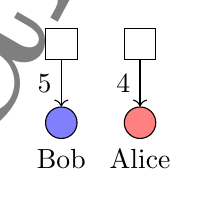
\begin{tikzpicture}[y=1cm, x=1cm]
        \node[sqadj] (a0) at (0, 0) {};
        \node[circB, label=below:Bob] (p0) at (0, -1) {};
        \node[sqadj] (a1) at (1, 0) {};
        \node[circA, label=below:Alice] (p1) at (1, -1) {};
        \draw[->] (a0) edge node[midway, left] { $5$ } (p0);
        \draw[->] (a1) edge node[midway, left] { $4$ } (p1);
      \end{tikzpicture}
    };

    \node (diag2) at (2, -2) {
      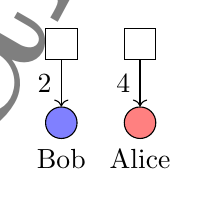
\begin{tikzpicture}[y=1cm, x=1cm]
        \node[sqadj] (a0) at (0, 0) {};
        \node[circB, label=below:Bob] (p0) at (0, -1) {};
        \node[sqadj] (a1) at (1, 0) {};
        \node[circA, label=below:Alice] (p1) at (1, -1) {};
        \draw[->] (a0) edge node[midway, left] { $2$ } (p0);
        \draw[->] (a1) edge node[midway, left] { $4$ } (p1);
      \end{tikzpicture}
    };

    \draw[->] (adj0) edge node[midway, above] { $D_\text{Alice}(4)$} (adj1);
    \draw[->] (adj1) edge node[midway, above] { $W_\text{Bob}(3)$} (adj2);
  \end{tikzpicture}
}
  \caption{
    Deposits and withdrawals.
    The deposit can be called by any blockchain user, provided that it is accompanied with a transfer of the same number of coins into the adjudicator.
    For the withdrawal to be successful, the withdrawal parameters must be signed with Bob's private key.
  }\label{fig:deposit-withdrawal}
\end{figure}

To recap, we now have a simple smart contract that can store a balance against an address, which either represents a participant or a channel.
The balances can be increased and decreased through deposits and withdrawals.
Anyone can deposit into an address of either type\footnote{But there is nothing to be gained from depositing into a participant address.} but funds can only be withdrawn from 
participant addresses - and only by a party who knows the private key.
The total coins held by the smart contract should always equal the sum of the balances.

\subsection{State Channel Outcomes}

In our model, a state channel is an off-chain protocol followed by a set of participants,
enabling them to reach an \textbf{outcome} that can be used to update the balances on the chain.
The format and interpretation of the outcome is specified by the state channel network protocol being used.
An example of a type of outcome is the \textit{allocation}, which is used in both Turbo and Nitro protocol, and which consists of a list of recipient addresses and totals that specify how the channel's balance should be distributed.

\begin{figure}[h]\centering
  \makebox[\textwidth][c]{\begin{tikzpicture}[x=1cm,y=1cm]
  \node[draw=black, rounded corners=0.5cm, outer sep=0.2cm] (adj0) at (0, 0) {
    \begin{tabular}{c|c|c}
      \multicolumn{3}{c}{\textbf{Adjudicator}} \\
      Address & Balance & Outcome \\
      \hline
      $L$ & $5$ & $A$: 1, $B$: 2 \\
      $L'$ & $6$ & \\
      $L''$ &  & $A$: 3, $B$: 4 \\
    \end{tabular}
  };

  \node (not0) at (3, -2.4) { $\adj{\holds{\text{L}}{5}{\alloc{A:1, B:2}}, \;\holds{L'}{6}{}, \; \holds{L''}{}{\alloc{A:3,B:4}}}$ };

  \node (diag0) at (7, 0) {
    \begin{tikzpicture}[y=1cm, x=1.5cm]
      \node[sqadj] (adj0) at (0, 0) {};
      \node[circAB, label=left:$L$] (L) at (0, -1) {};
      \draw[->] (adj0) edge node[midway, left] { $5$ } (L);
      \node[circA, label=below:$A$] (LA) at (-0.5, -2) {};
      \node[circB, label=below:$B$] (LB) at (0.5, -2) {};
      \draw[->] (L) edge node[midway, left] { $1$ } (LA);
      \draw[->] (L) edge node[midway, right] { $2$ } (LB);

      \node[sqadj] (a1) at (1, 0) {};
      \node[circAB, label=below:$L'$] (p1) at (1, -1) {};
      \draw[->] (a1) edge node[midway, left] { $6$ } (p1);

      \node[circAB, label=right:$L''$] (L'') at (2, -1) {};
      \node[circA, label=below:$A$] (L''A) at (1.5, -2) {};
      \node[circB, label=below:$B$] (L''B) at (2.5, -2) {};
      \draw[->] (L'') edge node[midway, left] { $3$ } (L''A);
      \draw[->] (L'') edge node[midway, right] { $4$ } (L''B);
    \end{tikzpicture}
  };

\end{tikzpicture}
}
  \caption{
    Representation of (allocation) outcomes in the three different diagram formats.
    We show the three possible cases: a channel, $L$, with both a balance and an outcome;
    a channel, $L'$, with a balance but no outcome; 
    and a channel, $L''$, with an outcome but no balance.
    We represent the channels with split circles, coloured to represent the participants of the channel, which we have taken to be $A$ and $B$.
  }\label{fig:outcome-notation}
\end{figure} 

Central to the approach of the model is to split the updating of the balances into two steps:
\begin{enumerate}
\item \textbf{Finalization}: getting to a point where the outcome of the channel is stored on the blockchain.
\item \textbf{Redistribution}: updating the balances in the adjudicator according to that outcome.
\end{enumerate}

The bulk of this paper is focussed on the redistribution step, which we will discuss further in section \ref{sec:redistribution}.

Understanding how an outcome is finalized inevitably involves understanding the rules of operation of the state channel: from exchanging states to launching and responding to challenges.
The ForceMove protocol completely specifies these rules of operation, in a way that is compatible with the work in this paper.

\begin{figure}[h]\centering
  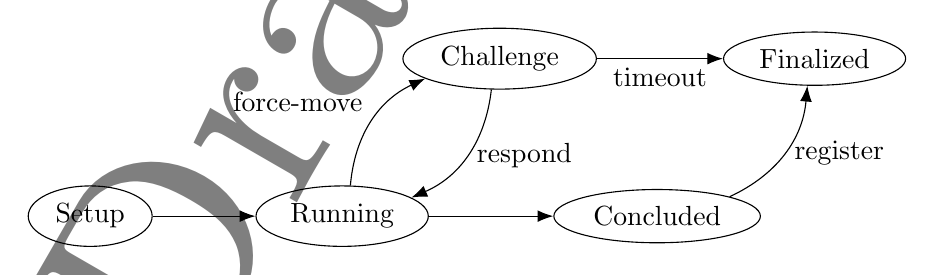
\begin{tikzpicture}[x=4cm,y=2cm]
  \tikzstyle{every node}=[draw, ellipse]

  % Specification of nodes (position, etc.)
  \node (Setup) at (-0.8,0) {Setup};
  \node (Running) at (0,0) {Running};
  \node (Concluded) at (1, 0) {Concluded};
  \node (Challenge) at (0.5, 1) {Challenge};
  \node (Finalized) at (1.5, 1) {Finalized};

  \begin{scope}[-{Latex[length=2mm]}]
    \tikzstyle{every node}=[draw=none,below]
    \draw (Setup) to (Running);
    \draw (Running) to (Concluded);
    \draw (Concluded) edge[bend right] node[midway, right] {register} (Finalized);
    \draw (Running) edge[bend left] node[midway,above left] {force-move} (Challenge) ;
    \draw (Challenge) edge[bend left] node[right] {respond} (Running);
    \draw (Challenge) edge node[midway, below] {timeout} (Finalized) ;
  \end{scope}
\end{tikzpicture}


  \caption{
    ForceMove Channel Operation. There are two ways for an outcome to become finalized: (i) through a challenge that times out before anyone responds, and (ii) through the registration of a conclusion proof.
  }\label{fig:modes}
\end{figure}

In ForceMove, there are two ways for an outcome to be finalized.
The first corresponds to a non-collaborative closing of the channel:
one participant launches an on-chain challenge, starting a timeout period;
if no other participant responds during the timeout period, then the challenge times out and the outcome
corresponding to the challenge state is finalized.
The second corresponds to a collaborative closing of the channel:
all the participants sign a special conclude state, called a conclusion proof; 
any participant can then register this outcome on-chain to create a finalized outcome.
By closing the channel collaboratively the participants avoid having to wait for the challenge period.

For the purpose of the model, it is crucial that the rules of operation only allow one outcome to be finalized for each channel.
As we will see in section \ref{sec:reasoning}, it is also important that the rules of operation make it possible to know which outcome(s) a participant can finalize from a given state.

\subsection{Redistribution}\label{sec:redistribution}

The second part of extracting the funds from a state channel is the redistribution step.
Redistribution involves calling a sequence of on-chain \textbf{operations} to manipulate
the balances and finalized outcomes.
The allowed operations are defined by the network protocol used.
Figure \ref{fig:redistribution} shows an example of the transfer operation from Turbo protocol.

\begin{figure}[h]\centering
  \makebox[\textwidth][c]{
\begin{tikzpicture}[x=8cm, y=2cm]
  \node[draw=black, rounded corners=0.5cm] (adj0) at (0, 0) {
    \begin{tabular}{c|c|c}
      \multicolumn{3}{c}{\textbf{Adjudicator}} \\
      Address & Balance & Outcome \\
      \hline
      L & 5 & Bob: 2, Alice: 3 \\
      Bob & 4 \\

    \end{tabular}
  };

  \node[draw=black, rounded corners=0.5cm] (adj0) at (1, 0) {
    \begin{tabular}{c|c|c}
      \multicolumn{3}{c}{\textbf{Adjudicator}} \\
      Address & Balance & Outcome \\
      \hline
      L & 5 & Bob: 2 \\
      Bob & 4 \\
      Alice & 3 \\
    \end{tabular}
  };

  \node (not0) at (0, -1) { $\adj{\holds{L}{5}{\alloc{\text{Bob}: 2, \text{Alice}: 3}}, \;\holds{\text{Bob}}{4}{}}$ };
  \node (not0) at (1, -1) { $\adj{\holds{L}{5}{\alloc{\text{Bob}: 2}}, \;\holds{\text{Bob}}{4}{}, \; \holds{\text{Alice}}{3}{}}$ };

  \node (diag0) at (0, -2) {
    \begin{tikzpicture}[y=1cm, x=2cm]
      \node[sqadj] (a0) at (0, 0) {};
      \node[circB, label=below:Bob] (p0) at (0, -1) {};
      \draw[->] (a0) edge node[midway, left] { $4$ } (p0);

      \node[sqadj] (a0) at (1, 0) {};
      \node[circAB, label=right:L] (p0) at (1, -1) {};
      \node[circB, label=below:Bob] (p1) at (0.58, -2) {};
      \node[circA, label=below:Alice] (p2) at (1.42, -2) {};


      \draw[->] (a0) edge node[midway, left] { $5$ } (p0);
      \draw[->] (p0) edge node[midway, left] { $2$ } (p1);
      \draw[->] (p0) edge node[midway, left] { $3$ } (p2);

    \end{tikzpicture}
  };

  \node (diag1) at (1, -2) {
    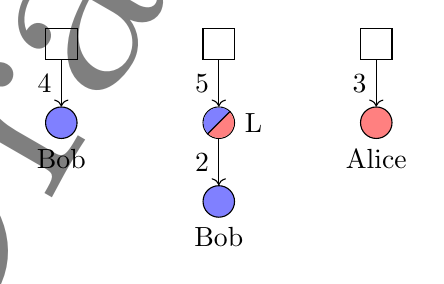
\begin{tikzpicture}[y=1cm, x=2cm]
      \node[sqadj] (a0) at (0, 0) {};
      \node[circB, label=below:Bob] (p0) at (0, -1) {};
      \draw[->] (a0) edge node[midway, left] { $4$ } (p0);

      \node[sqadj] (a1) at (1, 0) {};
      \node[circAB, label=right:L] (pab) at (1, -1) {};
      \node[circB, label=below:Bob] (pabb) at (1, -2) {};
      \draw[->] (a1) edge node[midway, left] { $5$ } (pab);
      \draw[->] (pab) edge node[midway, left] { $2$ } (pabb);

      \node[sqadj] (a2) at (2, 0) {};
      \node[circA, label=below:Alice] (pa) at (2, -1) {};
      \draw[->] (a2) edge node[midway, left] { $3$ } (pa);

    \end{tikzpicture}
  };
\end{tikzpicture}
}
  \caption{
    A example of a redistribution operation from Turbo protocol.
    Here the transfer operation is used to move $3$ coins out of channel $L$ to Alice.
    Note: the parts of the adjudicator responsible for storing challenges are omitted from the diagram.
  }\label{fig:redistribution}
\end{figure}

The operations change the state of the adjudicator: typically both balances and outcomes.
There is no restriction on who can trigger the operations.
In this paper, we present all operations separately and assume they are called separately.
In practice, we expect that implementations would provide some utility methods that combine
common sequences of operations, to improve gas efficiency.

To recap, we now have a system where participants can deposit into state channel addresses on-chain.
By running a state channel, participants can reach an outcome and ensure this outcome is finalized on-chain.
Once the outcome is finalized, the funds held in the channel can be redistributed to other participants and channels by calling on-chain operations.
Participants can then withdraw any funds that have been redistributed to their address.

In the next section, we will use this model to develop some tools for constructing state channel networks and proving their safety.
In particular, we will develop the logic which allows us to use the fact that a given outcome could be finalized if necessary, to avoid putting that outcome on-chain at all.

\section{Reasoning about State Channels}\label{sec:reasoning}

In this section, we outline our approach to proving the correctness of our state channel network constructions.

The very nature of state channels tends to make the logic complex.
In a state channel, value is moved between participants by exchanging commitments about the distribution of assets held on-chain.
Inevitably you end up reasoning about the commitments you hold and their interpretation by the chain, which necessarily also includes reasoning about the possible actions of the other parties both internal and external to the channel.

On top of this, there is an inherent danger in entering into a state channel relationship, as it requires funds to be locked on-chain.
In order to be safe, protocols need to be robust against other parties acting maliciously and/or ceasing to cooperate at any point in the protocol.
We need to show that at any point, any participant can extract the value currently owed to them in spite of any actions taken by other parties.

\subsection{Channel Funding and Value}

We will start by considering the interpretation of the outcome of a state channel.
Suppose $A$ is a participant in a state channel, $L$, that reaches an (allocation) outcome, $\omega$, that allocates $x$ coins to $A$.
What does that mean for $A$?
In particular, how much more can $A$ withdraw from the system due to that outcome?

\begin{figure}[h]\centering
  \makebox[\textwidth][c]{\begin{tikzpicture}[node distance=0.3cm]
  \node (outcome) at (0, 0) {
    \begin{tikzpicture}[x=0.7cm]
      \node[circAB, label=right:$L$] (L) at (0, 0) {};
      \node[circA, label=below:$A$] (A) at (-1, -1) {};
      \node[circB, label=below:$B$] (B) at (1, -1) {};
      \draw[->] (L) edge node[midway, left] { $3$ } (A);
      \draw[->] (L) edge node[midway, right] { $4$ } (B);
    \end{tikzpicture}
  };
  \node[right=of outcome] (plus) {$+$};
  \node[right=of plus] (otherstuff) {$\dots$};
  \node[right=2cm of otherstuff] (balance) {
    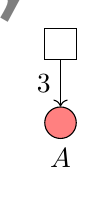
\begin{tikzpicture}
      \node[sqadj] (adj) at (0, 0) {};
      \node[circA, label=below:$A$] (A) at (0, -1) {};
      \draw[->] (adj) edge node[midway, left] { $3$ } (A);
    \end{tikzpicture}
  };
  \draw[shorten <=0.5cm, shorten >=0.3cm, -{Latex[length=2mm]}] (otherstuff) edge node[midway, above] { ? } (balance);
  \node[right=of balance] (plus2) {$+$};
  \node[right=of plus2] {$\dots$};
\end{tikzpicture}
}
  \caption{
    Understanding whether a channel is funded amounts to understanding how much value can be extracted from the system when that channel reaches an outcome.
  }\label{fig:meaning-of-funding}
\end{figure}

There is one case where the answer to these questions is very straightforward:
where the channel $L$ itself has enough coins in the adjudicator to cover the entire allocation.
In this case, we say the channel is \textbf{directly funded}.
If this happens, $A$ will receive all $x$ coins allocated to them in $\omega$.
\begin{figure}[h]\centering
  \makebox[\textwidth][c]{\begin{tikzpicture}[node distance=2cm]
  \node (diag0) {
    \begin{tikzpicture}[y=1cm, x=2cm]
      \node[sqadj] (a0) at (1, 0) {};
      \node[circAB, label=right:$L$] (p0) at (1, -1) {};
      \node[circA, label=below:$A$] (p1) at (0.58, -2) {};
      \node[circB, label=below:$B$] (p2) at (1.42, -2) {};

      \draw[->] (a0) edge node[midway, left] { $7$ } (p0);
      \draw[->] (p0) edge node[midway, left] { $3$ } (p1);
      \draw[->] (p0) edge node[midway, right] { $4$ } (p2);

    \end{tikzpicture}
  };

  \node[right=of diag0] (diag1) {
    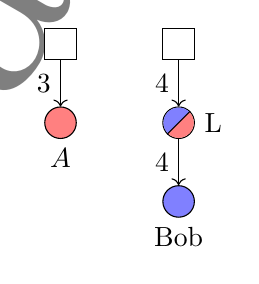
\begin{tikzpicture}[y=1cm, x=1.5cm]
      \node[sqadj] (a0) at (0, 0) {};
      \node[circA, label=below:$A$] (p0) at (0, -1) {};
      \draw[->] (a0) edge node[midway, left] { $3$ } (p0);

      \node[sqadj] (a1) at (1, 0) {};
      \node[circAB, label=right:L] (pab) at (1, -1) {};
      \node[circB, label=below:Bob] (pabb) at (1, -2) {};
      \draw[->] (a1) edge node[midway, left] { $4$ } (pab);
      \draw[->] (pab) edge node[midway, left] { $4$ } (pabb);
    \end{tikzpicture}
  };

  \draw[shorten <=0.5cm, shorten >=0.3cm, -{Latex[length=2mm]}] (diag0) to (diag1);
\end{tikzpicture}
}
  \caption{
    Direct funding.
    One case where we know we can extract the full value allocated to us in a channel outcome, is when the channel has a sufficient balance in the adjudicator to cover the full allocation.
  }\label{fig:direct-funding}
\end{figure}

This is a good start, but the whole point of state channel \textit{networks} is to move beyond the case where every channel needs to be directly funded.
Suppose instead that $L$ is not directly funded but there is another channel, $L'$, that is.
Further suppose that $L'$ has reached an outcome where all its coins are allocated to $L$.
Using this outcome, we know we can redistribute the coins in the adjudicator to $L$, recreating the situation above, where $L$ was directly funded.
Therefore, in this situation we also know that $A$ will receive the $x$ coins from the outcome of $L$, and that $L$ can be considered to be \textbf{indirectly funded}.
Note that we did not actually need to perform the redistribution on-chain to reach this conclusion - we just needed to be able to reason that the outcome enabled us to.

\begin{figure}[h]\centering
  \makebox[\textwidth][c]{\begin{tikzpicture}[node distance=2cm]
  \node (diag0) {
    \begin{tikzpicture}[y=1cm, x=1.5cm]
      \node[sqadj] (a0) at (1, 1) {};
      \node[circAB, label=right:$L'$] (l0) at (1, 0) {};


      \node[circAB, label=right:$L'$] (l1) at (2, 0) {};
      \node[circAB, label=right:$L$] (p0) at (2, -1) {};

      \draw[->] (a0) edge node[midway, left] { $7$ } (l0);
      \draw[->] (l1) edge node[midway, left] { $7$ } (p0);

    \end{tikzpicture}
  };

  \node[right=of diag0] (diag1) {
    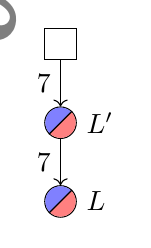
\begin{tikzpicture}[y=1cm, x=2cm]
      \node[sqadj] (a0) at (1, 1) {};
      \node[circAB, label=right:$L'$] (l0) at (1, 0) {};
      \node[circAB, label=right:$L$] (p0) at (1, -1) {};

      \draw[->] (a0) edge node[midway, left] { $7$ } (l0);
      \draw[->] (l0) edge node[midway, left] { $7$ } (p0);

    \end{tikzpicture}
  };

  \node[right=of diag1] (diag2) {
    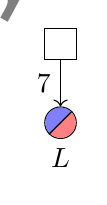
\begin{tikzpicture}[y=1cm, x=1.5cm]
      \node[sqadj] (a0) at (0, 0) {};
      \node[circAB, label=below:$L$] (p0) at (0, -1) {};
      \draw[->] (a0) edge node[midway, left] { $7$ } (p0);
    \end{tikzpicture}
  };

  \path[draw=none] (diag0) -- node (b) {\Large $\equiv$ } (diag1);
  \draw[shorten <=0.5cm, shorten >=0.3cm, -{Latex[length=2mm]}] (diag1) to (diag2);
\end{tikzpicture}
}
  \caption{
    Indirect funding.
    If we possess another outcome, that allocates funds to $L$, we know we can convert this to a situation where $L$ is directly funded.
    We can therefore consider $L$ to be indirectly funded.
  }\label{fig:indirect-funding}
\end{figure}

In the previous paragraph, we looked at the case where $L'$ had already reached an outcome.
In general, this will not be the case;
the power of state channels comes from the ability to move between many potential outcomes as the interaction progresses.
In order to say whether a channel is funded, we will need to start not with an outcome but with a \textbf{network state}.
The network state, $\Sigma$, for a participant, $A$, consists of:
\begin{enumerate}
  \item The state of the adjudicator: 
  \begin{enumerate}
    \item The balances held
    \item Any finalized outcomes
  \end{enumerate}
  \item For each channel $A$ is a partipicant of:
  \begin{enumerate}
    \item Signed commitments that $A$ has received
    \item Signed commitments that $A$ has sent
    \item Private information held by $A$
  \end{enumerate}
\end{enumerate}
The private information always includes $A$'s signing key for the channel and can also include information specific to the application running in the channel;
for example, in a game of battleships the private information would include the positions of $A$'s ships.
Note that $A$'s network state does not include a detailed model of which commitments are held by specific other participants - just what $A$ has sent and received.
Generally we assume that all other participants are controlled by a single adversary, pooling their resources and commitments. 

\begin{figure}[h]\centering
  \makebox[\textwidth][c]{\begin{tikzpicture}[node distance=2cm]
  \node[cloud, draw,cloud puffs=10,cloud puff arc=120, aspect=2, inner ysep=1em, align=center] (systemstate) {$\Sigma$};

  \node[right=of systemstate] (diag0) {
    \begin{tikzpicture}[y=1cm, x=2cm]
      \node[sqadj] (a0) at (1, 0) {};
      \node[circAB, label=right:$L$] (p0) at (1, -1) {};
      \node[circA, label=below:$A$] (p1) at (0.58, -2) {};
      \node[circB, label=below:$B$] (p2) at (1.42, -2) {};

      \draw[->] (a0) edge node[midway, left] { $7$ } (p0);
      \draw[->] (p0) edge node[midway, left] { $3$ } (p1);
      \draw[->] (p0) edge node[midway, right] { $4$ } (p2);

    \end{tikzpicture}
  };

  \node[right=of diag0] (diag1) {
    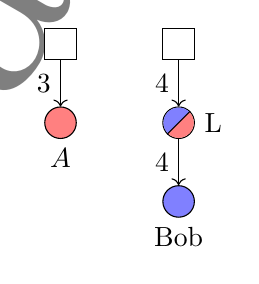
\begin{tikzpicture}[y=1cm, x=1.5cm]
      \node[sqadj] (a0) at (0, 0) {};
      \node[circA, label=below:$A$] (p0) at (0, -1) {};
      \draw[->] (a0) edge node[midway, left] { $3$ } (p0);

      \node[sqadj] (a1) at (1, 0) {};
      \node[circAB, label=right:L] (pab) at (1, -1) {};
      \node[circB, label=below:Bob] (pabb) at (1, -2) {};
      \draw[->] (a1) edge node[midway, left] { $4$ } (pab);
      \draw[->] (pab) edge node[midway, left] { $4$ } (pabb);
    \end{tikzpicture}
  };

  \draw[shorten <=0.5cm, shorten >=0.3cm, -{Latex[length=2mm]}] (systemstate) to (diag0);
  \draw[shorten <=0.5cm, shorten >=0.3cm, -{Latex[length=2mm]}] (diag0) to (diag1);
\end{tikzpicture}
}
  \caption{
    In practice, we deal with a network state, $\Sigma$, and not in definite outcomes.
    To understand value, we also need to be able to reason about which outcome(s) could result from the current network state, as well as the value those outcomes then deliver.
  }\label{fig:system-state-direct-funding}
\end{figure}

We can now proceed with some definitions of funding and value:

A channel $\rchi$ is \textbf{funded} for participant $A$ with $x$ coins, if $A$ has an unbeatable strategy for obtaining a state where $\rchi$ is directly funded with $x$ coins.

The $\textbf{value}$ for participant $A$ of a network state $\Sigma$ is the maximum $x$ for which $A$ has an unbeatable strategy for obtaining a state where the balance of $A$'s address in the adjudicator is $x$ coins.

The concept of an unbeatable strategy can involve a full range of actions allowed within the protocol including signing commitments, refusing to sign commitments, launching/responding to on-chain challenges and calling on-chain operations to redistribute funds.
We will cover this in more detail in section \ref{sec:unbeatable-strategy}.

\subsection{Network Constructions}

Now that we have defined what we mean by a channel being funded and a state having value, we can start to talk about the state channel network constructions that will form the bulk of the paper.
A construction specifies both the network state for each participant and a sequence of states that can be used to reach it.
Presenting a construction will follow the same rough pattern:
\begin{enumerate}
  \item Show that a given network state funds a channel.
  \item Show it can be built from a known state, using a sequence of value-preserving single channel updates.
\end{enumerate}
The single channel update requirement is a key decision in the design the protocol.
This means that we do not allow atomic updates across multiple channels;
each update to the system comprises sending or receiving a single statement applying to just one channel.
This keeps channel updates independent, which makes it a lot easier to reason about finalizability on a per-channel basis.

We require that the sequence of state transitions is value preserving for each participants involved. 
While the power of state channel networks comes from being able to move value off-chain, opening and closing channels can be viewed as rewriting the existing state in a different form and therefore should not change the value.
We furthermore make the assumption that participants will be willing to make any transition that preserves their value, meaning that value-preservation is both a necessary and sufficient property for constructing network states.
We call this last assumption the \textbf{Simple Transition Rule}. 

In the case where we ignore the cost of the on-chain redistribution operations, the simple transition rule is straightforward and non-controversial.
If we consider this cost, the situation becomes a bit more subtle, as moving from a simpler to a more complicated construction actually leads to a slight decrease the value that is extractable from the network.
In practice, using the simple transition rule means we are assuming that the utility from being able to fund channels off-chain will outweigh the slight increase in cost in the worst-case scenario.
Modelling the cost of the on-chain operations is beyond the scope of this paper.

\subsection{Unbeatable Strategies}\label{sec:unbeatable-strategy}

In the definitions of value and funding, we talked about having an unbeatable strategy for obtaining some state on-chain.
The means that whatever actions (or lack of actions) other participants and external parties might take, the target state is still obtainable.
This is not the easiest definition to work with:
to show that a strategy is unbeatable it seems that you have to consider all possible actions other parties could take.
In this section, we will break this down and give some tools to make it easier to show that a strategy is unbeatable.

We start by outlining the rules for interacting with the blockchain.
When evaluating whether a strategy is unbeatable, we make the following assumptions about blockchain transactions:
\begin{enumerate}
  \item \textbf{Transactions are unimpeded}: given that the current time is $t$ and $\epsilon > 0$, then it is possible for any party to apply any operation, $O$, on-chain before time $t + \epsilon$.
  \item \textbf{Transactions \textit{can} be front-run}: given two parties, $p_1$ and $p_2$, and two operations, $O_1$ and $O_2$, there is no way for $p_1$ to ensure that they can apply $O_1$ to the chain before $p_2$ applies $O_2$.
\end{enumerate}
The first assumption sidesteps issues of censorship, chain congestion and timing considerations around the creation of blocks.
In practice, this assumption should hold if $\epsilon$ is sufficiently large, which can be accomplished by picking sensible channel timeouts.
The second assumption rules out any strategies that rely on executing a given transaction on-chain before someone else executes a different one.

We now take the task of constructing an unbeatable strategy and break it into two stages: finalization and redistribution. 

Finalization happens on a per-channel basis, with different channels finalizing independently.
This makes it easier to reason about which outcomes are possible.
In general, we cannot assume that the outcome will be known;
we might have to take multiple possible outcomes through to the redistribution step.
\begin{figure}[h]\centering
  \makebox[\textwidth][c]{\begin{tikzpicture}[x=5cm, y=2cm]
  \node[cloud, draw,cloud puffs=10,cloud puff arc=120, aspect=2, inner ysep=1em, align=center] (systemstate) at (0,0) {$\Sigma$};

  \node (opt0) at (1.2, 1) {
    \begin{tikzpicture}[y=1cm, x=2cm]
      \node[sqadj] (a0) at (1, 0) {};
      \node[circAB, label=right:$L$] (p0) at (1, -1) {};
      \node[circA, label=below:$A$] (p1) at (0.58, -2) {};
      \node[circB, label=below:$B$] (p2) at (1.42, -2) {};

      \draw[->] (a0) edge node[midway, left] { $7$ } (p0);
      \draw[->] (p0) edge node[midway, left] { $3$ } (p1);
      \draw[->] (p0) edge node[midway, right] { $4$ } (p2);

    \end{tikzpicture}
  };
   
  % \node (opt2) at (1, 0) {$\vdots$ };

  \node (opt1) at (0.9, -1) {
    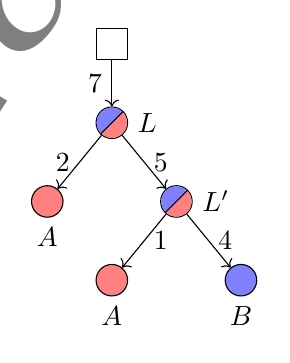
\begin{tikzpicture}[y=1cm, x=0.82cm]
      \node[sqadj] (a0) at (1, 0) {};
      \node[circAB, label=right:$L$] (p0) at (1, -1) {};
      \node[circA, label=below:$A$] (p1) at (0, -2) {};
      \node[circAB, label=right:$L'$] (p2) at (2, -2) {};
      \node[circA, label=below:$A$] (p3) at (1, -3) {};
      \node[circB, label=below:$B$] (p4) at (3, -3) {};

      \draw[->] (a0) edge node[midway, left] { $7$ } (p0);
      \draw[->] (p0) edge node[midway, left] { $2$ } (p1);
      \draw[->] (p0) edge node[midway, right] { $5$ } (p2);
      \draw[->] (p2) edge node[midway, right] { $1$ } (p3);
      \draw[->] (p2) edge node[midway, right] { $4$ } (p4);

    \end{tikzpicture}
  };

  \node (val) at (2, 0) {
    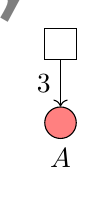
\begin{tikzpicture}[y=1cm, x=1.5cm]
      \node[sqadj] (a0) at (0, 0) {};
      \node[circA, label=below:$A$] (p0) at (0, -1) {};
      \draw[->] (a0) edge node[midway, left] { $3$ } (p0);
    \end{tikzpicture}
  };

  \draw[shorten <=0.5cm, shorten >=0.3cm, -{Latex[length=2mm]}] (systemstate) to (opt0);
  \draw[shorten <=0.5cm, shorten >=0.3cm, -{Latex[length=2mm]}] (systemstate) to (opt1);
  % \draw[shorten <=0.5cm, shorten >=0.3cm, -{Latex[length=2mm]}] (systemstate) to (opt2);
  \draw[shorten <=0.5cm, shorten >=0.3cm, -{Latex[length=2mm]}] (opt0) to (val);
  \draw[shorten <=0.5cm, shorten >=0.3cm, -{Latex[length=2mm]}] (opt1) to (val);
  % \draw[shorten <=0.5cm, shorten >=0.3cm, -{Latex[length=2mm]}] (opt2) to (val);
\end{tikzpicture}
}
  \caption{When calculating value, we will often need to consider all outcomes that are possible from a given network state and show that they all allow us to extract the same value from the network.}
\end{figure}
The finalization step depends heavily on the rules of the state channel framework.
We will cover finalization in more detail in section \ref{sec:finalizable-outcomes}.

Reasoning about when a redistribution strategy is unbeatable, depends heavily on the protocol involved. 
We will cover the logic here in the sections on Turbo and Nitro protocol.
In Turbo, it turns out that the answer is simple: any strategy that works is unbeatable.
In Nitro, it is more complicated to show that redistribution strategies are unbeatable but we provide a few tools to help.

\subsection{Finalizable Outcomes}\label{sec:finalizable-outcomes}

We say an outcome, $\Omega$, is \textbf{finalizable} for participant $A$, if $A$ has an unbeatable
strategy for finalizing this outcome in the adjudicator.
We use the notation $\finalizable{\rchi}{\Omega}{A}$, to represent a state of a channel, $\rchi$,
where the outcome, $\Omega$, is finalizable by $A$.
\begin{align}
  \finalizable{\rchi}{\Omega}{A} \xrightarrow{\text{A's unbeatable strategy}} \adj{\holds{\rchi}{}{\Omega}}
\end{align}

It follows from the definition that exactly one of the following statements is true about
a channel $\rchi$ at any point in time:
\begin{enumerate}
  \item Finalized outcome: the outcome of $\rchi$ has already been finalized on-chain: $\adj{\holds{\rchi}{}{\Omega}}$
  \item One participant has multiple finalizable outcomes: participant $p$ has one or more finalizable outcome(s), $\Omega_1, \dots, \Omega_m$, and no other participant has any finalizable outcomes.
        We write this $\finalizable{\rchi}{\Omega_1, \dots, \Omega_m}{p}$.
  \item Multiple participants share one finalizable outcome: there are at least two participants, $P = \{p_1, \dots, p_m \}$, who share the same
        finalizable outcome, $\Omega$. We write this $\finalizable{\rchi}{\Omega}{p_1, \dots, p_m}$.
  \item No finalizable outcomes: there are no participants with any finalizable outcomes.
\end{enumerate}
The definition of finalizability excludes the case where two different finalizable outcomes are held
by different participants, as in this case at least one participant's strategy would be beatable
by the other participant's strategy.
None of the protocols we present make use of the last case, where no participant has a finalizable outcome.

\begin{figure}[h]\centering
  \makebox[\textwidth][c]{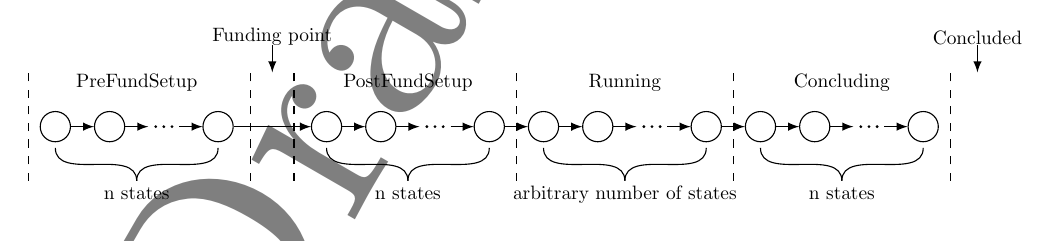
\begin{tikzpicture}[x=28pt,y=28pt,scale=0.7, every node/.style={transform shape}]
  \newcommand{\paperdiagram}[3]{%
    \begin{scope}[shift={(#1,0)}]
      % Circle
      \foreach \n in {0,1,3} {\node[circle,draw,text width=10pt,inner sep=0pt] (N\n#1) at (\n,0) {\strut};}
      % Transparent circle
      \foreach \n in {2} {\node[circle,draw,text width=10pt,inner sep=0pt,white] (N\n#1) at (\n,0) {\strut};}
      % Dots
      \foreach \n in {1.85,2,2.15} {\fill (\n,0) circle (0.8pt);}
      % Arrows
      \foreach \x [remember=\x as \lastx (initially 0)] in {1,2,3}{\draw[-latex] (N\lastx#1) -- (N\x#1);}
      % Under brackets with label #3
      \foreach \n in {0,3} {\draw ([shift={(0,-3pt)}]N\n#1.south) to[out=270,in=90] (1.5,-1) node[inner sep=1pt] (P) {\strut};}
      \node at (P.south) {\strut#3};
      % Upper label #2
      \node at (1.5,0.8) {\strut#2};
    \end{scope}
  }
  % Diagram nodes
  \paperdiagram{0}{PreFundSetup}{n states}
  \paperdiagram{5}{PostFundSetup}{n states}
  \paperdiagram{9}{Running}{arbitrary number of states}
  \paperdiagram{13}{Concluding}{n states}
  % Arrows between single diagram node
  \foreach \x [remember=\x as \lastx (initially 0)] in {5,9,13}{\draw[-latex] (N3\lastx) -- (N0\x);}
  % Vertical dashed
  \foreach \n in {-0.5,3.6,4.4,8.5,12.5,16.5} {\draw[dashed] (\n,-1) --++(90:2);}
  % Funding arrow
  \draw[latex-] (4,1) --++(90:0.5) node[at end,above,inner sep=0pt] {Funding point};
  \draw[latex-] (17,1) --++(90:0.5) node[at end,above,inner sep=0pt] {Concluded};
\end{tikzpicture}
}
  \caption{
    Every ForceMove channel has at least two points when the outcome is universally finalizable: one at the funding point and one when the channel has concluded.
    This is important when reasoning about creating state channel network constructions.
  }
\end{figure}
In the special case where the outcome of a channel is finalizable by all its participants, we say that the outcome is \textbf{universally finalizable}.
For a ForceMove channel, this happens at the following points in its lifecycle:
\begin{enumerate}
  \item After the first $n$ states have been broadcast. In this state, we say the channel is at the \textbf{funding point}.
  \item When a single conclusion proof is known to each participant. In this state, we say the channel is in the \textbf{concluded state}.
\end{enumerate}
It is an important property of ForceMove that all channels have one universally finalizable
state at the beginning of their lifecycle and one at the end\footnote{If a channel does not end with a conclusion proof, it ends with an expired on-chain challenge,
in which case the outcome is already finalized on-chain.}.

If a participant has no finalizable outcomes, their analysis of the network needs to be performed
in terms of their \textbf{enabled outcomes}.
The enabled outcomes for a participant, $p$, is defined as the set of outcomes that $p$ has
no strategy to prevent from being finalized.
We write the set of enabled outcomes for $p$ as $\finalizable{\rchi}{\Omega_1 \dots \Omega_m}{(p)}$.

For any participant, $p$, in a channel, $\rchi$, exactly one of the following statements is
true at a given point in time:
\begin{enumerate}
  \item $p$ has at least one finalizable outcome.
  \item $p$ has at least two enabled outcomes.
\end{enumerate}
Note that if a participant has only enabled a single outcome, that outcome must be finalizable for them.

\subsection{Consensus Game}

Another important example of universally finalizable states comes from the \textbf{consensus game}.
The consensus game is a ForceMove \textit{application}, which means it specifies a certain
set of transitions rules that can be used to define the allowed state transitions for a ForceMove channel.
We will make heavy use of the consensus game throughout the paper.

The consensus game provides a way for participants to move from one universally finalizable outcome to another, provided that they all agree.
The participants start in a state where $\Omega_1$ is the universally finalizable outcome.
One participant proposes the new outcome, $\Omega_2$.
On their turn, each subsequent participant decides whether to accept the transition to the new outcome or whether to cancel the transition and return to $\Omega_1$.
\begin{figure}[h]\centering
  \makebox[\textwidth][c]{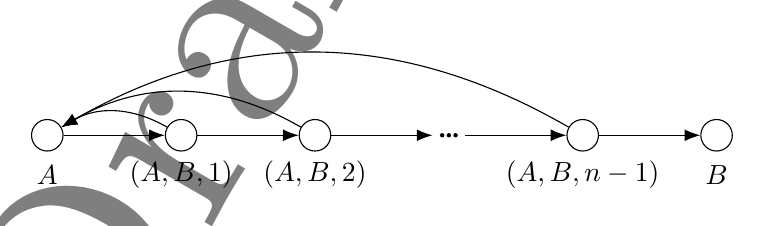
\begin{tikzpicture}[x=1.7cm, y=1cm]
  \begin{scope}[every node/.style={draw,circle,minimum size=4mm}]
    \node (A) at (0,0) {};
    \node (AB1) at (1,0) {};
    \node (AB2) at (2,0) {};
    \node[draw=none] (ABx) at (3,0) {};
    % Dots
    \foreach \n in {2.95,3,3.05} {\fill (\n,0) circle (0.8pt);}
    \node (ABn) at (4,0) {};
    \node (B) at (5,0) {};
  \end{scope}
  \begin{scope}
    \node at ([yshift=-0.5cm]A) { $A$ };
    \node at ([yshift=-0.5cm]AB1) { $(A, B, 1)$ };
    \node at ([yshift=-0.5cm]AB2) { $(A, B, 2)$ };
    \node at ([yshift=-0.5cm]ABn) { $(A, B, n-1)$ };
    \node at ([yshift=-0.5cm]B) { $B$ };
  \end{scope}
  \begin{scope}[-{Latex[length=2mm]}]
    \draw (A) to (AB1);
    \draw (AB1) to (AB2);
    \draw (AB2) to (ABx);
    \draw (ABx) to (ABn);
    \draw (ABn) to (B);
    \draw (AB1) to[bend right] (A);
    \draw (AB2) to[bend right] (A);
    \draw (ABn) to[bend right] (A);
  \end{scope}
\end{tikzpicture}
}
  \caption{
    A consensus game transition from $\Omega_1$ to $\Omega_2$, for a channel with $n$ participants.
    The counter records how many participants have approved the transition.
    If all participants agree, they finish in a state with outcome $\Omega_2$.
    Any participant can reject the transition, returning to the state with $\Omega_1$.
  }
\end{figure}

Throughout the only enabled outcomes for any participant are $\Omega_1$ and $\Omega_2$.
In particular, a participant has the finalizable outcome $\finalizable{\rchi}{\Omega_1}{p}$ until they approve the transition, and then enabled outcomes $\finalizable{\rchi}{\Omega_1, \Omega_2}{(p)}$ until they receive the final state.
When the final state is broadcast, every participant has the finalizable outcome $\finalizable{\rchi}{\Omega_2}{p}$.

\subsection{Outcomes First}

In practice, it is hard to write networks states down concisely.
Instead, we will write our constructions in terms of outcomes and use the properties of the consensus game to reason that (a) network states exist that lead to this outcome and (b) we can find a sequence of network states to transition from one outcome to another.

In particular, we will present sequences of sets of outcomes, where each set differs only in the outcome of a single consensus game channel.
Each of the outcomes will have the same value to all participants.
We then know that, using the properties of the consensus game, we can transition between these two states with a consensus game transition, without enabling any additional outcomes.

To show that we can build a construction, it is therefore sufficient to present the sequence of sets of equal-value outcomes, where each set differs only in the outcome of a single consensus game channel. This is the approach we will take in the rest of the paper.

\begin{figure}[h]\centering
  \makebox[\textwidth][c]{\begin{tikzpicture}[node distance=1cm]
  \node (s0) {
    \begin{tikzpicture}[x=0.7cm]
      \node[circAB, label=right:$L$] (L) at (0, 0) {};
      \node[circA, label=below:$A$] (A) at (-1, -1) {};
      \node[circB, label=below:$B$] (B) at (1, -1) {};
      \draw[->] (L) edge node[midway, left] { $3$ } (A);
      \draw[->] (L) edge node[midway, right] { $4$ } (B);
    \end{tikzpicture}
  };
  \node[right=of s0.south east, anchor=south west] (s1) {
    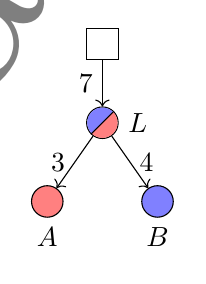
\begin{tikzpicture}[y=1cm, x=0.7cm]
      \node[sqadj] (a0) at (1, 0) {};
      \node[circAB, label=right:$L$] (p0) at (1, -1) {};
      \node[circA, label=below:$A$] (p1) at (0, -2) {};
      \node[circB, label=below:$B$] (p2) at (2, -2) {};

      \draw[->] (a0) edge node[midway, left] { $7$ } (p0);
      \draw[->] (p0) edge node[midway, left] { $3$ } (p1);
      \draw[->] (p0) edge node[midway, right] { $4$ } (p2);

    \end{tikzpicture}
  };

  \node[right=of s1.north east, anchor = north west] (s2) {
    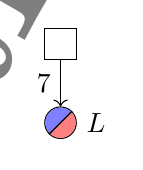
\begin{tikzpicture}[y=1cm, x=2cm]
      \node[sqadj] (a0) at (1, 0) {};
      \node[circAB, label=right:$L$] (p0) at (1, -1) {};

      \draw[->] (a0) edge node[midway, left] { $7$ } (p0);

    \end{tikzpicture}
  };

  \node[right=of s2.north east, anchor=north west] (s3) {
    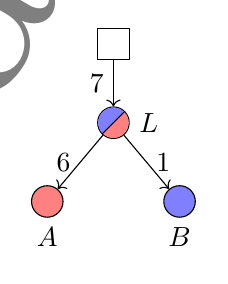
\begin{tikzpicture}[y=1cm, x=2cm]
      \node[sqadj] (a0) at (1, 0) {};
      \node[circAB, label=right:$L$] (p0) at (1, -1) {};
      \node[circA, label=below:$A$] (p1) at (0.58, -2) {};
      \node[circB, label=below:$B$] (p2) at (1.42, -2) {};

      \draw[->] (a0) edge node[midway, left] { $7$ } (p0);
      \draw[->] (p0) edge node[midway, left] { $6$ } (p1);
      \draw[->] (p0) edge node[midway, right] { $1$ } (p2);

    \end{tikzpicture}
  };

  \node[right=of s3.north east, anchor=north west] (s4) {
    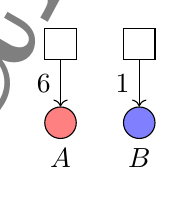
\begin{tikzpicture}[y=1cm, x=1cm]
      \node[sqadj] (a0) at (1, 0) {};
      \node[circA, label=below:$A$] (p0) at (1, -1) {};
      \node[sqadj] (a1) at (2, 0) {};
      \node[circB, label=below:$B$] (p1) at (2, -1) {};

      \draw[->] (a0) edge node[midway, left] { $6$ } (p0);
      \draw[->] (a1) edge node[midway, left] { $1$ } (p1);

    \end{tikzpicture}
  };
  \node (mid) at ([yshift=-3mm] s0.north) {};
  \begin{scope}[-{Latex[length=2mm]}]
    \draw (s0.east |- mid) to (s1.west |- mid);
    \draw (s1.east |- mid) to (s2.west |- mid);
    \draw (s2.east |- mid) to (s3.west |- mid);
    \draw (s3.east |- mid) to (s4.west |- mid);
  \end{scope}

  \node[below=-1mm of s0] (below) { (a) };
  \node at (s1 |- below) { (b) };
  \node at (s2 |- below) { (c) };
  \node at (s3 |- below) { (d) };
  \node at (s4 |- below) { (e) };
\end{tikzpicture}
}
  \caption{
    In (a), $A$ and $B$ have exchanged the first two states in the channel $L$, bringing them to the funding point. At this point the channel is not yet funded.
    In step (b), both participants have deposited into the adjudicator.
    In step (c), the channel $L$ is running.
    $A$ and $B$ do not have a finalizable outcome and the ultimate outcome is governed by the rules given by the channel's game library.
    In step (d), $A$ and $B$ have created a conclusion proof and therefore have another universally finalizable outcome.
    They are then able to finalize this outcome on-chain and withdraw their funds in (e).
  }
\end{figure}



% \section{Turbo Protocol}

Turbo protocol has one type of outcome (the allocation) and one on-chain operation (the transfer).
You will already be somewhat familiar with these, as they formed the basis of a lot of the examples in sections \ref{sec:modelling} and \ref{sec:reasoning}.
In this section we will make these more precise, present the related result on distribution and give some example constructions to cover common tasks such as opening and closing sub-channels.

\subsection{Allocations and Transfer}

An \textbf{allocation} is a list of pairs of addresses and totals, $\alloc{a_1{:}v_1, \dots, a_m{:}v_m}$, where each total, $v_i$, represents that quantity of coins due to each address, $a_i$.
We assume that each address only appears once in the allocation and require that implementations enforce this by ignoring any additional entries for a given address after the first.

The allocation is in priority order, so that if the channel does not hold enough funds to pay all the coins that are due, then the addresses at the beginning of the allocation will receive funds first.
We say that `$A$ \textbf{can afford} $x$ for $B$', if $B$ would receive at least $x$ coins, were the coins currently held by $A$ to be paid out in priority order.

\begin{figure}[h]\centering
  \makebox[\textwidth][c]{\begin{tikzpicture}[x=6.5cm, y=2cm]
  \node (diag0) at (0, 0) {
    \begin{tikzpicture}[y=1cm, x=2cm]

      \node[sqadj] (a0) at (1, 0) {};
      \node[circAB, label=right:$L$] (p0) at (1, -1) {};
      \node[circB, label=below:$B$] (p1) at (0.58, -2) {};
      \node[circA, label=below:$A$] (p2) at (1.42, -2) {};

      \draw[->] (a0) edge node[midway, left] { $5$ } (p0);
      \draw[->] (p0) edge node[midway, left] { $4$ } (p1);
      \draw[->] (p0) edge node[midway, right] { $3$ } (p2);

    \end{tikzpicture}
  };

  \node (diag1) at (1, 0) {
    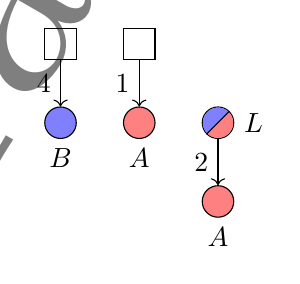
\begin{tikzpicture}[y=1cm, x=1cm]
      \node[sqadj] (a0) at (0, 0) {};
      \node[circB, label=below:$B$] (p0) at (0, -1) {};
      \draw[->] (a0) edge node[midway, left] { $4$ } (p0);

      \node[sqadj] (a2) at (1, 0) {};
      \node[circA, label=below:$A$] (pa) at (1, -1) {};
      \draw[->] (a2) edge node[midway, left] { $1$ } (pa);

      \node[circAB, label=right:$L$] (p1) at (2, -1) {};
      \node[circA, label=below:$A$] (p2) at (2, -2) {};
      \draw[->] (p1) edge node[midway, left] { $2$ } (p2);
    \end{tikzpicture}
  };

  \draw[shorten <=0.5cm, shorten >=0.3cm, -{Latex[length=2mm]}] (diag0) edge node[midway, above] {$\transfer{L}{B}{4}\; \transfer{L}{A}{1}$} (diag1);
\end{tikzpicture}
}
  \caption{
    Allocations pay out in priority order.
    In the diagram, $B$ is drawn to the left of $A$ to show that $B$ has higher priority in the outcome of $L$.
    In this example, $L$ can afford $4$ coins for $B$, but can only afford $1$ coin for $A$.
  }\label{fig:transfer-insufficient-funds}
\end{figure}

Turbo introduces the \textbf{transfer} operation, $\transfer{A}{B}{x}$, to trigger the on-chain transfer of funds according to an allocation.
If $A$ can afford $x$ for $B$, then $\transfer{A}{B}{x}$:
\begin{enumerate}
  \item Reduces the funds held in channel $A$ by $x$. 
  \item Increases the funds held by $B$ by $x$.
  \item Reduces the amount owed to $B$ in the outcome of $A$ by $x$.
\end{enumerate}
If $A$ cannot afford $x$ for $B$, then $\transfer{A}{B}{x}$ fails, leaving the on-chain state unchanged.

\subsection{Unbeatable Redistribution}

As we mentioned in section \ref{sec:unbeatable-strategy}, reasoning about redistribution is easy in Turbo: if you can find one strategy to move a certain amount into an address, then no-one else can prevent this from occurring.
In this section we will justify this by presenting an algorithm for calculating the funding for each address.

We will restrict ourselves to looking at strategies and counter-strategies involving transfer operations only, ignoring deposits and withdrawals.
We claim that deposits and withdrawals cannot be required as part of a strategy and cannot help as part of a counter-strategy.
The intuition here is that a deposit into the system cannot reduce the value of any address and cannot increase the value of any address by more than the value of the deposit.
Withdrawals can only occur from participant addresses and are the only way funds can leave these addresses, so cannot affect values elsewhere.

We will consider the network of outcomes to be a directed acylcic graph (DAG), where the nodes are channels and the edges represent allocations from one channel to the other.
While it is technically possible to create outcomes with cycles, it is also possible for any participant in the channel to prevent this from happening.
We therefore consider non-DAG outcome networks to be outside the scope of the protocol.

We commence our value calculation by taking a \textit{topological ordering} of the nodes of the graph.
A topological ordering is an ordering the nodes such that, if $N_1 \mapsto N_2$ is an edge, then $N_1 < N_2$.
It is a known result that all DAGs have at least one topological ordering.

\begin{figure}[h]\centering
  \makebox[\textwidth][c]{\begin{tikzpicture}
\node (s1) {
  \begin{tikzpicture}[y=1cm, x=1cm]
    \node[sqadj] (adj) at (0, 0) {};
    \node[circAB, label=right:$L$] (L) at (0, -1) {};
    \node[circA, label=below:$A$] (A) at (-1, -2) {};
    \node[circB, label=below:$B$] (B) at (0, -2) {};
    \node[circAB, label=right:$\rchi$] (chi) at (1, -2) {};
    \draw[->] (adj) edge node[midway, left] { $7$ } (L);

    \draw[->] (L) edge node[midway, left] { $3$ } (A);
    \draw[->] (L) edge node[midway, right] { $1$ } (B);
    \draw[->] (L) edge node[midway, right] { $6$ } (chi);

    \node[circA, label=below:$A$] (chiA) at (0.4, -3) {};
    \node[circB, label=below:$B$] (chiB) at (1.6, -3) {};

    \draw[->] (chi) edge node[midway, right] { $2$ } (chiA);
    \draw[->] (chi) edge node[midway, right] { $4$ } (chiB);
  \end{tikzpicture}
};

\node[right=of s1] (s2) {
  \begin{tikzpicture}[y=1cm, x=1cm]
    \node[sqadj] (adj) at (0, 0) {};
    \node[valuebox, label=right:$L$] (L) at (0, -1) { 1 \nodepart{second}  };
    \node[valuebox, label=right:$\rchi$] (chi) at (1, -2) { 2};
    \draw[->] (adj) edge node[midway, left] { $7$ } (L);

    \draw[->] (L) edge node[midway, right] { $6$ } (chi);

    \node[valuebox, label=below:$A$] (chiA) at (-1, -3) {3};
    \node[valuebox, label=below:$B$] (chiB) at (0.5, -3) {4};

    \draw[->] (chi) edge node[near end, above] { $2$ } (chiA);
    \draw[->] (chi) edge node[midway, right] { $4$ } (chiB);
    \draw[->] (L) edge node[midway, left] { $3$ } (chiA);
    \draw[->] (L) edge node[near start, right] { $1$ } (chiB);
  \end{tikzpicture}
};

\node[right=of s2] (s3) {
  \begin{tikzpicture}[y=1cm, x=1cm]
    \node[sqadj] (adj) at (0, 0) {};
    \node[valuebox, label=right:$L$] (L) at (0, -1) { 1 \nodepart{second} 7 };
    \node[valuebox, label=right:$\rchi$] (chi) at (1, -2) { 2 \nodepart{second} 3};
    \draw[->] (adj) edge node[midway, left] { $7$ } (L);

    \draw[->] (L) edge node[midway, right] { $6$ } (chi);

    \node[valuebox, label=below:$A$] (chiA) at (-1, -3) {3 \nodepart{second} 5};
    \node[valuebox, label=below:$B$] (chiB) at (0.5, -3) {4 \nodepart{second} 2};

    \draw[->] (chi) edge node[near end, above] { $2$ } (chiA);
    \draw[->] (chi) edge node[midway, right] { $4$ } (chiB);
    \draw[->] (L) edge node[midway, left] { $3$ } (chiA);
    \draw[->] (L) edge node[near start, right] { $1$ } (chiB);
  \end{tikzpicture}
};
\node[below=-1mm of s1] (below) { (a) };
\node at (s2 |- below) { (b) };
\node at (s3 |- below) { (c) };
\end{tikzpicture}







}
  \caption{
    Diagram (a) shows the outcome network that is the input to the value calculation.
    In (b), we have reformulated (a) as a DAG with uniquely labelled nodes by merging the two $A$ and $B$ modes.
    We have also labelled the nodes with a topological ordering.
    In (c), we have completed the algorithm giving each node its funding/value.
  }\label{fig:turbo-redistribution}
\end{figure}

Once we have ordered the nodes, we work through the nodes in order.
For a node, $n$, we first look at the amount of direct funding allocated to $n$'s address in the adjudicator.
We then look at each of $n$'s parents and calculate the amount that that the parent can afford for $n$, according to the value of the parent (which will already have been calculated, due to the topological ordering).
Finally we set the node's value to be the sum of the direct funding and the amounts afforded by each parent.

\textbf{Turbo Value Algorithm}
\begin{enumerate}
  \item Choose a topological ordering, \texttt{OrderedNodes}, for the network.
  \item Create a mapping, \texttt{Values}, from \texttt{OrderedNodes} to $\mathbb{Z}^+$. Initialize this mapping by setting $\texttt{Values}[n]$ to be the balance held for $n$ in the adjudicator, for each $n \in \texttt{OrderedNodes}$ (with $\texttt{Values}[n] = 0$ if $n$'s address does not appear).
  \item For each $n \in \texttt{OrderedNodes}[n]$ (taken in order):
  \begin{enumerate}
    \item Let $\texttt{remainingFunds} = \texttt{Values}[n]$.
    \item For each $(\texttt{destinationNode}, \texttt{payout})$ in $n$'s allocation (taken in order):
      \begin{enumerate}
        \item Let $x = \text{min}(\texttt{payout}, \texttt{remainingFunds})$.
        \item Increase $\texttt{Values}[\texttt{destinationNode}]$ by $x$.
        \item Decrease $\texttt{remainingFunds}$ by $x$.
      \end{enumerate}
  \end{enumerate}
  \item Then $\texttt{Values}[n]$ gives the value of node $n$.
\end{enumerate}




It is not hard to see that it is impossible to find a strategy that gives any node a value higher than allocated by this algorithm.
It also is not hard to construct a strategy for a node to obtain the value allocated by the algorithm, if necessary by actually implementing the algorithm up until that node.
Given that we are only considering counter-strategies with transfers, and we have done every possible transfer on these channels, we know that there are no transfers that can interrupt this algorithm.
It is also easy to see that calling transfers out of order does not affect the ultimate result.

In Turbo, it is therefore easy to calculate the value of each node and find unbeatable strategies for extracting the value of that address .

\subsection{Ledger Channels}

A \textbf{ledger} channel is a channel whose sole purpose is to provide funding to other channels.
We call the channels that are funded by the ledger channel \textbf{sub-channels} of the ledger channel.
All ledger channels run the consensus game.

Although this has already been covered, for completeness we will quickly recap how a sub-channel can be considered to be funded by a ledger channel.
For example, consider the following setup where a ledger channel, $L$, allocates the funds it holds to participants $A$ and $B$ and channel $\rchi$:
\begin{align}
  \adj{\holds{L}{10}{}}, \finalizable{L}{\alloc{A: 3, B: 1, \rchi: 6}}{A, B}
\end{align}
\begin{figure}[h]\centering
  \makebox[\textwidth][c]{\begin{tikzpicture}[node distance=2cm]
  \node (s1) {
    \begin{tikzpicture}[y=1cm, x=1cm]
      \node[sqadj] (adj) at (0, 0) {};
      \node[circAB, label=right:$L$] (L) at (0, -1) {};
      \node[circA, label=below:$A$] (A) at (-1, -2) {};
      \node[circB, label=below:$B$] (B) at (0, -2) {};
      \node[circAB, label=right:$\rchi$] (chi) at (1, -2) {};
      \draw[->] (adj) edge node[midway, left] { $10$ } (L);
  
      \draw[->] (L) edge node[midway, left] { $3$ } (A);
      \draw[->] (L) edge node[midway, right] { $1$ } (B);
      \draw[->] (L) edge node[midway, right] { $6$ } (chi);
  
    \end{tikzpicture}
  };

  \node[right=of s1] (s2) {
    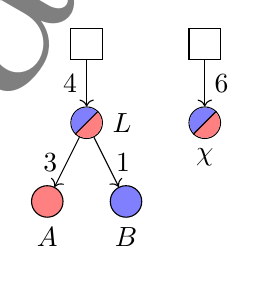
\begin{tikzpicture}[y=1cm, x=1cm]

      \node[sqadj] (adj) at (0, 0) {};
      \node[circAB, label=right:$L$] (L) at (0, -1) {};
      \node[circA, label=below:$A$] (A) at (-0.5, -2) {};
      \node[circB, label=below:$B$] (B) at (0.5, -2) {};
      \draw[->] (adj) edge node[midway, left] { $4$ } (L);
  
      \draw[->] (L) edge node[midway, left] { $3$ } (A);
      \draw[->] (L) edge node[midway, right] { $1$ } (B);
  
      \node[sqadj] (adj2) at (1.5, 0) {};
      \node[circAB, label=below:$\rchi$] (chi) at (1.5, -1) {};
      \draw[->] (adj2) edge node[midway, right] { $6$ } (chi);
    \end{tikzpicture}
  };

  \draw[-{Latex[length=2mm]}] (s1) edge node[midway, above] {$\transfer{L}{\rchi}{6}$} (s2);
\end{tikzpicture}
}
  \caption{
    Offloading a ledger channel.
  }\label{fig:ledger-offload}
\end{figure}
In this example, $\rchi$ is funded with 6 coins by $L$ for both $A$ and $B$.
To show this, we have to have an unbeatable strategy for moving to a situation where $\rchi$ is directly funded with 6 coins.
To do this we first note that the outcome $\alloc{A: 3, B: 1, \rchi: 6}$ is finalizable for both $A$ and $B$, so we can start our strategy by putting this outcome on-chain.
Once it is on-chain, the transfer operation $\transfer{L}{\rchi}{6}$ is all that is required to make $\rchi$ directly funded.
From the Turbo redistribution result, we know that this redistribution strategy is unbeatable.

Note that offloading $\rchi$ like this should be seen as an action of last-resort, as after the off-load all sub-channels supported by $L$ to be closed on-chain.
It is in the interest of both participants to open and close sub-channels collaboratively.
We next give some examples to show how this can be accomplished safely.

\subsection{Example Constructions}

We now give some examples of how to work with ledger channels on Turbo.
We have chosen to present examples that demonstrate the key principles instead of presenting general protocols, as we believe that, once seen, these protocols are easy to extend to the general case.

\subsubsection{Opening a Sub-channel}

\begin{figure}[h]\centering
  \makebox[\textwidth][c]{\begin{tikzpicture}[x=4cm]
  \node[draw] (s0) at (0, 0) {
    \begin{tikzpicture}[y=1cm, x=1.2cm]
      \node[sqadj] (adj) at (0, 0) {};
      \node[circAB, label=right:$L$] (L) at (0, -1) {};
      \node[circA, label=below:$A$] (A) at (-0.5, -2) {};
      \node[circB, label=below:$B$] (B) at (0.5, -2) {};
      \node[circle, draw=none, label=below:\strut] at (0, -3) {}; %ghost node for alignment%
      \draw[->] (adj) edge node[midway, left] { $10$ } (L);
      \draw[->] (L) edge node[midway, left] { $5$ } (A);
      \draw[->] (L) edge node[midway, right] { $5$ } (B);
    \end{tikzpicture}
  };

  \node[right=of s0] (s1) {
    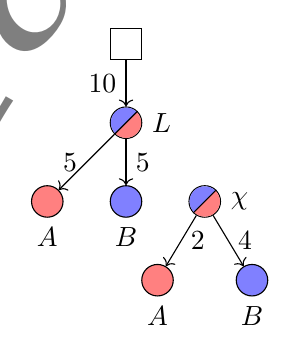
\begin{tikzpicture}[y=1cm, x=1cm]
      \node[sqadj] (adj) at (0, 0) {};
      \node[circAB, label=right:$L$] (L) at (0, -1) {};
      \node[circA, label=below:$A$] (A) at (-1, -2) {};
      \node[circB, label=below:$B$] (B) at (0, -2) {};
      \node[circAB, label=right:$\rchi$] (chi) at (1, -2) {};
      \draw[->] (adj) edge node[midway, left] { $10$ } (L);
      \draw[->] (L) edge node[midway, left] { $5$ } (A);
      \draw[->] (L) edge node[midway, right] { $5$ } (B);

      \node[circA, label=below:$A$] (chiA) at (0.4, -3) {};
      \node[circB, label=below:$B$] (chiB) at (1.6, -3) {};

      \draw[->] (chi) edge node[midway, right] { $2$ } (chiA);
      \draw[->] (chi) edge node[midway, right] { $4$ } (chiB);
    \end{tikzpicture}
  };

  \node[right=of s1.north east, anchor=north west] (s2) {
    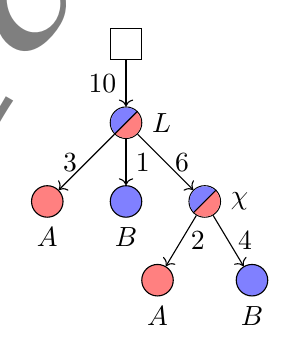
\begin{tikzpicture}[y=1cm, x=1cm]
      \node[sqadj] (adj) at (0, 0) {};
      \node[circAB, label=right:$L$] (L) at (0, -1) {};
      \node[circA, label=below:$A$] (A) at (-1, -2) {};
      \node[circB, label=below:$B$] (B) at (0, -2) {};
      \node[circAB, label=right:$\rchi$] (chi) at (1, -2) {};
      \draw[->] (adj) edge node[midway, left] { $10$ } (L);

      \draw[->] (L) edge node[midway, left] { $3$ } (A);
      \draw[->] (L) edge node[midway, right] { $1$ } (B);
      \draw[->] (L) edge node[midway, right] { $6$ } (chi);

      \node[circA, label=below:$A$] (chiA) at (0.4, -3) {};
      \node[circB, label=below:$B$] (chiB) at (1.6, -3) {};

      \draw[->] (chi) edge node[midway, right] { $2$ } (chiA);
      \draw[->] (chi) edge node[midway, right] { $4$ } (chiB);
    \end{tikzpicture}
  };

  \node[right=of s2.north east, anchor=north west] (s3) {
    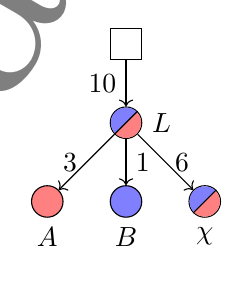
\begin{tikzpicture}[y=1cm, x=1cm]
      \node[sqadj] (adj) at (0, 0) {};
      \node[circAB, label=right:$L$] (L) at (0, -1) {};
      \node[circA, label=below:$A$] (A) at (-1, -2) {};
      \node[circB, label=below:$B$] (B) at (0, -2) {};
      \node[circAB, label=below:$\rchi$] (chi) at (1, -2) {};
      \draw[->] (adj) edge node[midway, left] { $10$ } (L);
      \draw[->] (L) edge node[midway, left] { $3$ } (A);
      \draw[->] (L) edge node[midway, right] { $1$ } (B);
      \draw[->] (L) edge node[midway, right] { $6$ } (chi);
    \end{tikzpicture}
  };

  \begin{scope}[shorten <=1cm, shorten >=1.4cm, -{Latex[length=2mm]}]
    \node (level) at (0, 0.8) {};
    \draw (s0 |- level) to (s1 |- level);
    \draw (s1 |- level) to (s2 |- level);
    \draw (s2 |- level) to (s3 |- level);
  \end{scope}
\end{tikzpicture}
}
  \caption{
  }\label{fig:opening-sub-channel}
\end{figure}

The utility of a ledger channel derives from the ability to open and close sub-channels without on-chain operations.
Here we show how to open a sub-channel.
\begin{enumerate}
  \item Start in a state where $A$ and $B$ have a funded ledger channel, $L$, open:
  \begin{align}
    \adj{\holds{L}{x}{}}, \; \finalizable{L}{\alloc{A: a, B: b}}{A, B}
  \end{align}
  \item $A$ and $B$ prepare their sub-channel $\rchi$ and progress it to the funding point. With $a' \leq a$ and $b' \leq b$:
  \begin{align}
    \finalizable{\rchi}{\alloc{A:a', B:b'}}{A,B}
  \end{align}
  \item Update the ledger channel to fund the sub-channel:
  \begin{align}
    \finalizable{L}{\alloc{A:a-a', B: b - b', \rchi: a' + b'}}{A,B}
  \end{align}
\end{enumerate}

\subsubsection{Closing a Sub-channel}

\begin{figure}[h]\centering
  \makebox[\textwidth][c]{\begin{tikzpicture}[x=4cm]
  \node (s0) at (0, 0) {
    \begin{tikzpicture}[y=1cm, x=1cm]
      \node[sqadj] (adj) at (0, 0) {};
      \node[circAB, label=right:$L$] (L) at (0, -1) {};
      \node[circA, label=below:$A$] (A) at (-1, -2) {};
      \node[circB, label=below:$B$] (B) at (0, -2) {};
      \node[circAB, label=below:$\rchi$] (chi) at (1, -2) {};
      \node[circle, draw=none, label=below:\strut] at (0, -3) {}; %ghost node for alignment%
      \draw[->] (adj) edge node[midway, left] { $10$ } (L);
      \draw[->] (L) edge node[midway, left] { $3$ } (A);
      \draw[->] (L) edge node[midway, right] { $1$ } (B);
      \draw[->] (L) edge node[midway, right] { $6$ } (chi);
    \end{tikzpicture}
  };

  \node[right=of s0] (s1) {
    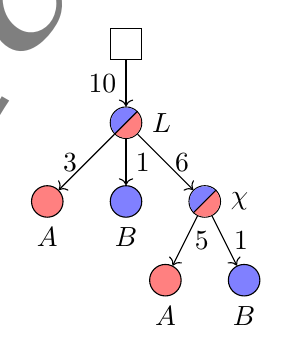
\begin{tikzpicture}[y=1cm, x=1cm]
      \node[sqadj] (adj) at (0, 0) {};
      \node[circAB, label=right:$L$] (L) at (0, -1) {};
      \node[circA, label=below:$A$] (A) at (-1, -2) {};
      \node[circB, label=below:$B$] (B) at (0, -2) {};
      \node[circAB, label=right:$\rchi$] (chi) at (1, -2) {};
      \draw[->] (adj) edge node[midway, left] { $10$ } (L);

      \draw[->] (L) edge node[midway, left] { $3$ } (A);
      \draw[->] (L) edge node[midway, right] { $1$ } (B);
      \draw[->] (L) edge node[midway, right] { $6$ } (chi);

      \node[circA, label=below:$A$] (chiA) at (0.5, -3) {};
      \node[circB, label=below:$B$] (chiB) at (1.5, -3) {};

      \draw[->] (chi) edge node[midway, right] { $5$ } (chiA);
      \draw[->] (chi) edge node[midway, right] { $1$ } (chiB);
    \end{tikzpicture}
  };

  \node[right=of s1] (s2) {
    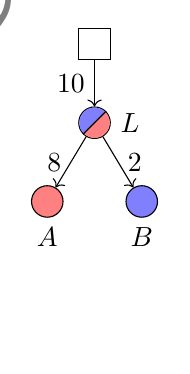
\begin{tikzpicture}[y=1cm, x=1.2cm]
      \node[sqadj] (adj) at (0, 0) {};
      \node[circAB, label=right:$L$] (L) at (0, -1) {};
      \node[circA, label=below:$A$] (A) at (-0.5, -2) {};
      \node[circB, label=below:$B$] (B) at (0.5, -2) {};
      \node[circle, draw=none, label=below:\strut] at (0, -3) {}; %ghost node for alignment%
      \draw[->] (adj) edge node[midway, left] { $10$ } (L);
      \draw[->] (L) edge node[midway, left] { $8$ } (A);
      \draw[->] (L) edge node[midway, right] { $2$ } (B);
    \end{tikzpicture}
  };

  \begin{scope}[shorten <=1cm, shorten >=1.4cm, -{Latex[length=2mm]}]
    \node (level) at (0, 0.8) {};
    \draw (s0 |- level) to (s1 |- level);
    \draw (s1 |- level) to (s2 |- level);
  \end{scope}
\end{tikzpicture}
}
  \caption{
  }\label{fig:closing-sub-channel}
\end{figure}

When the interaction in a sub-channel, $\rchi$, has finished we need a safe way to update the ledger channels to incorporate the outcome.
This allows the sub-channel to be defunded and closed off-chain.
\begin{enumerate}
  \item We start in the state where $\rchi$ is funded via the ledger channel, $L$. With $x = a + b + c$:
  \begin{align}
    \adj{\holds{L}{x}{}}, \; \finalizable{L}{\alloc{A: a, B: b, \rchi: c}}{A, B}
  \end{align}
  \item The next step is for $A$ and $B$ to concluded channel $\rchi$, leaving the channel in the conclude state. Assuming $a' + b' = c$:
  \begin{align}
    \finalizable{\rchi}{\alloc{A:a', B:b'}}{A,B}
  \end{align}
  \item The participants then update the ledger channel to include the result of channel $\rchi$.
  \begin{align}
    \finalizable{L}{\alloc{A: a+ a', B: b + b'}}{A, B}
  \end{align}
  \item Now the sub-channel $\rchi$ has been defunded, it can be safely discarded.
\end{enumerate}

\subsubsection{Topping Up a Ledger Channel}

\begin{figure}[h]\centering
  \makebox[\textwidth][c]{\begin{tikzpicture}[x=4cm]
  \node (s0) at (0, 0) {
    \begin{tikzpicture}[y=1cm, x=1cm]
      \node[sqadj] (adj) at (0, 0) {};
      \node[circAB, label=right:$L$] (L) at (0, -1) {};
      \node[circA, label=below:$A$] (A) at (-1, -2) {};
      \node[circB, label=below:$B$] (B) at (0, -2) {};
      \node[circAB, label=below:$\rchi$] (chi) at (1, -2) {};
      \draw[->] (adj) edge node[midway, right] { 10 } (L);
      \draw[->] (L) edge node[pos=0.6, left=1mm] { 7 } (A);
      \draw[->] (L) edge node[pos=0.7, left=-0mm] { 1 } (B);
      \draw[->] (L) edge node[pos=0.6, right=1mm] { 2 } (chi);
    \end{tikzpicture}
  };

  \node (s1) at (1, 0) {
    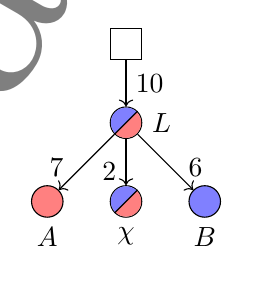
\begin{tikzpicture}[y=1cm, x=1cm]
      \node[sqadj] (adj) at (0, 0) {};
      \node[circAB, label=right:$L$] (L) at (0, -1) {};
      \node[circA, label=below:$A$] (A) at (-1, -2) {};
      \node[circAB, label=below:$\rchi$] (chi) at (0, -2) {};
      \node[circB, label=below:$B$] (B) at (1, -2) {};
      \draw[->] (adj) edge node[midway, right] { 10 } (L);
      \draw[->] (L) edge node[pos=0.6, left=1mm] { 7 } (A);
      \draw[->] (L) edge node[pos=0.7, left=-0mm] { 2 } (chi);
      \draw[->] (L) edge node[pos=0.6, right=1mm] { 6 } (B);
    \end{tikzpicture}
  };

  \node (s2) at (2, 0) {
    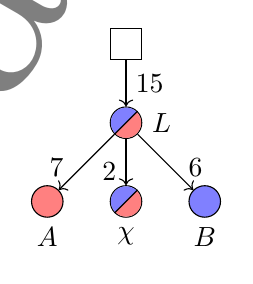
\begin{tikzpicture}[y=1cm, x=1cm]
      \node[sqadj] (adj) at (0, 0) {};
      \node[circAB, label=right:$L$] (L) at (0, -1) {};
      \node[circA, label=below:$A$] (A) at (-1, -2) {};
      \node[circAB, label=below:$\rchi$] (chi) at (0, -2) {};
      \node[circB, label=below:$B$] (B) at (1, -2) {};
      \draw[->] (adj) edge node[midway, right] { 15 } (L);
      \draw[->] (L) edge node[pos=0.6, left=1mm] { 7 } (A);
      \draw[->] (L) edge node[pos=0.7, left=-0mm] { 2 } (chi);
      \draw[->] (L) edge node[pos=0.6, right=1mm] { 6 } (B);
    \end{tikzpicture}
  };

  \node (s3) at (3, 0) {
    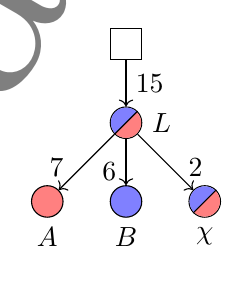
\begin{tikzpicture}[y=1cm, x=1cm]
      \node[sqadj] (adj) at (0, 0) {};
      \node[circAB, label=right:$L$] (L) at (0, -1) {};
      \node[circA, label=below:$A$] (A) at (-1, -2) {};
      \node[circB, label=below:$B$] (B) at (0, -2) {};
      \node[circAB, label=below:$\rchi$] (chi) at (1, -2) {};
      \draw[->] (adj) edge node[midway, right] { 15 } (L);
      \draw[->] (L) edge node[pos=0.6, left=1mm] { 7 } (A);
      \draw[->] (L) edge node[pos=0.7, left=-0mm] { 6 } (B);
      \draw[->] (L) edge node[pos=0.6, right=1mm] { 2 } (chi);
    \end{tikzpicture}
  };

  \begin{scope}[shorten <=1cm, shorten >=1.4cm, -{Latex[length=2mm]}]
    \node (level) at (0, 0.8) {};
    \draw (s0 |- level) to (s1 |- level);
    \draw (s1 |- level) to (s2 |- level);
    \draw (s2 |- level) to (s3 |- level);
  \end{scope}
\end{tikzpicture}
}
  \caption{
  }\label{fig:ledger-top-up}
\end{figure}

Here we show how a participant can increase their funds held in a ledger channel by depositing into it.
They can do this without disturbing any sub-channels supported by the ledger channel.
\begin{enumerate}
  \item In this process $A$ wants to deposit an additional $a'$ coins into the the ledger channel $L$. We start in the state where $L$ contains balances for $A$ and $B$, as well as funding a sub-channel, $\rchi$. With $x = a + b + c$:
  \begin{align}
    \adj{\holds{L}{x}{}}, \; \finalizable{L}{\alloc{A: a, B: b, \rchi: c}}{A, B}
  \end{align}
  \item To prepare for the deposit the participants update the state to move $A$'s entry to the end, simultaneously increasing $A$'s total. This is a safe operation due to the precedence rules: as the channel is currently underfunded $A$ would still only receive $a$ if the outcome went to chain.
  \begin{align}
    \finalizable{L}{\alloc{B:b, \rchi: c, A: a + a'}}{A,B}
  \end{align}
  \item It is now safe for $A$ to deposit into the channel on-chain:
  \begin{align}
    D_L(a')\adj{\holds{L}{x}{}} = \adj{\holds{L}{x + a'}{}}
  \end{align}
  \item Finally, if required, the participants can reorder the state again:
  \begin{align}
    \finalizable{L}{\alloc{ A: a + a', B: b, \rchi: c}}{A,B}
  \end{align}
\end{enumerate}

\subsubsection{Partial Withdrawal from a Ledger Channel}

A partial checkout is the opposite of a top up: 
one participant has excess funds in the ledger channel that they wish to withdraw on-chain.
The participants want to do this without disturbing any sub-channels supported by the ledger channels.

\begin{figure}[h]\centering
  \makebox[\textwidth][c]{\begin{tikzpicture}[x=4cm]
  \node (s0) at (0, 0) {
    \begin{tikzpicture}[y=1.2cm, x=1cm]
      \node[sqadj] (adj) at (0, 0) {};
      \node[circAB, label=right:$L$] (L) at (0, -1) {};
      \node[circA, label=below:$A$] (A) at (-1, -2) {};
      \node[circB, label=below:$B$] (B) at (0, -2) {};
      \node[circAB, label=below:$\rchi$] (chi) at (1, -2) {};
      \draw[->] (adj) edge node[midway, right] { 10 } (L);
      \draw[->] (L) edge node[near end, left=1mm] { 7 } (A);
      \draw[->] (L) edge node[near end, left] { 1 } (B);
      \draw[->] (L) edge node[near end, right=1mm] { 2 } (chi);
    \end{tikzpicture}
  };

  \node (s1) at (1, 0) {
    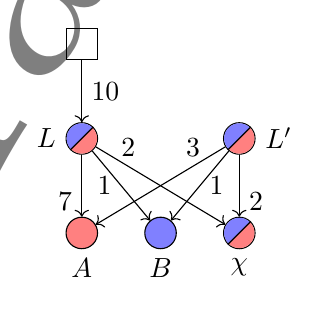
\begin{tikzpicture}[y=1.2cm, x=1cm]
      \node[sqadj] (adj) at (-1, 0) {};
      \node[circAB, label=left:$L$] (L) at (-1, -1) {};
      \node[circA, label=below:$A$] (A) at (-1, -2) {};
      \node[circB, label=below:$B$] (B) at (0, -2) {};
      \node[circAB, label=below:$\rchi$] (chi) at (1, -2) {};
      \draw[->] (adj) edge node[midway, right] { 10 } (L);
      \draw[->] (L) edge node[near end, left] { 7 } (A);
      \draw[->] (L) edge node[midway, left] { 1 } (B);
      \draw[->] (L) edge node[near start, above] { 2 } (chi);

      \node[circAB, label=right:$L'$] (Lp) at (1, -1) {};
      \draw[->] (Lp) edge node[near start, above] {3} (A);
      \draw[->] (Lp) edge node[midway, right] {1} (B);
      \draw[->] (Lp) edge node[near end, right] {2} (chi);

    \end{tikzpicture}
  };

  \node (s2) at (2, 0) {
    \begin{tikzpicture}[y=1.2cm, x=1cm]
      \node[sqadj] (adj) at (0, 0) {};
      \node[circAB, label=left:$L$] (L) at (0, -1) {};
      \node[circA, label=below:$A$] (A1) at (-1, -2) {};
      \node[circA, label=below:$A$] (A) at (0, -2) {};
      \node[circB, label=below:$B$] (B) at (1, -2) {};
      \node[circAB, label=below:$\rchi$] (chi) at (2, -2) {};
      \draw[->] (adj) edge node[midway, left] {10} (L);
      \draw[->] (L) edge node[near end, left=1mm] {4} (A1);
      \draw[->] (L) edge node[midway, above] {6} (Lp);

      \node[circAB, label=right:$L'$] (Lp) at (1, -1) { };
      \draw[->] (Lp) edge node[near end, left=1mm] { 3 } (A);
      \draw[->] (Lp) edge node[near end, left] { 1 } (B);
      \draw[->] (Lp) edge node[near end, right=1mm] { 2 } (chi);

    \end{tikzpicture}
  };

  \node (s3) at (3, 0) {
    \begin{tikzpicture}[y=1.2cm, x=1cm]

      \node[sqadj] (adj1) at (0, 0) {};
      \node[circA, label=below:$A$] (A1) at (0, -1) {};
      \draw[->] (adj) edge node[midway, right] {4 } (A1);

      \node[sqadj] (adj) at (1, 0) {};
      \node[circA, label=below:$A$] (A) at (0, -2) {};
      \node[circB, label=below:$B$] (B) at (1, -2) {};
      \node[circAB, label=below:$\rchi$] (chi) at (2, -2) {};
      \draw[->] (adj) edge node[midway, right] {6} (Lp);

      \node[circAB, label=right:$L'$] (Lp) at (1, -1) {};
      \draw[->] (Lp) edge node[near end, right] {3} (A);
      \draw[->] (Lp) edge node[near end, right] {1} (B);
      \draw[->] (Lp) edge node[near end, right=1mm] {2} (chi);

    \end{tikzpicture}
  };

  \begin{scope}[shorten <=1cm, shorten >=1.4cm, -{Latex[length=2mm]}]
    \node (level) at (0, 0.8) {};
    \draw (s0 |- level) to (s1 |- level);
    \draw (s1 |- level) to (s2 |- level);
    \draw (s2 |- level) to (s3 |- level);
  \end{scope}
\end{tikzpicture}
}
  \caption{Cool, huh?}
\end{figure}

\begin{enumerate}
  \item We start with a ledger channel, $L$, that $A$ wants to withdraw $a'$ coins from:
  \begin{align}
    \adj{\holds{L}{x}{}}, \; \finalizable{L}{\alloc{A: a + a', B: b, \rchi: c}}{A, B}
  \end{align}
  \item The participants start by preparing a new ledger channel, $L'$, whose state reflects the situation they want to be in after $A$ has withdrawn their coins. This is safe to do as this channel is currently unfunded.
  \begin{align}
    \finalizable{L'}{\alloc{A: a, B:b, \rchi: c}}{A,B}
  \end{align}
  \item They then update $L$ to fund $L'$ alongside the coins that $A$ wants to withdraw. They conclude the channel in this state:
  \begin{align}
    \finalizable{L}{\alloc{L': a + b + c, A: a'}}{A,B}
  \end{align}
  \item They then finalize the outcome of $L$ on-chain. This can be done without waiting the timeout, assuming they both signed the conclusion proof in the previous step:
  \begin{align}
    \adj{\holds{L}{x}{\alloc{L': a + b + c, A: a'}}}
  \end{align}
  \item $A$ can then call the transfer operation to get their coins under their control. 
  \begin{multline}
    \transfer{L}{A}{a'}\adj{\holds{L}{x}{\alloc{L: a + b + c, A: a'}}} = \\ \adj{\holds{L}{x - a'}{\alloc{L': a + b + c}}, \; \holds{A}{a}{}}
  \end{multline}
  \item At any point in the future the remaining coins can be transferred to $L'$:
  \begin{multline}
    \transfer{L}{L'}{a + b + c}\adj{\holds{L}{x}{\alloc{L: a + b + c}}, \; \holds{A}{a'}{}} =  \\ \adj{\holds{L'}{a + b + c}{}, \; \holds{A}{a'}{}}
  \end{multline}
\end{enumerate}
Note that $A$ was able to withdraw their funds instantly, without having to wait for the channel timeout.

% \section{Nitro Protocol}

Nitro protocol is an extension to Turbo protocol.
In Nitro protocol, the outcome of a channel can be either an allocation or a \textbf{guarantee}.
- operations can be a transfer or a claim

\subsection{Guarantees and Claims}

A guarantee outcome specifies the address of a target allocation channel; the protocol specifies how this guarantee may be used to pay debt on its behalf.
When paying debt, a guarantee can be used to alter the payout priority of the allocation outcome of its target address. 

\begin{tikzpicture}[y=0.8cm]
  \node[semicircle, draw] (upper) at (0,0) {};
  \node[semicircle, draw, rotate=180] (lower) at (0,-1) {};

  \draw[-] (upper.220) to (lower.320);
  \draw[-] (upper.270) to (lower.270);
  \draw[-] (upper.320) to (lower.220);

  \node[semicircle, draw] (upper1) at (1,0) {};
  \node[semicircle, draw, rotate=180] (lower1) at (1,-1) {};

  \draw[-] (upper1.220) to[out=270, in=90] (lower1.270);
  \draw[-] (upper1.270) to[out=270, in=90] (lower1.220);
  \draw[-] (upper1.320) to[out=270, in=90] (lower1.320);

  \pic (A) at (2, -0.5) {guarantee};
\end{tikzpicture}

We will use the notation $\guar{L}{A_1, A_2, \dots, A_m}$ for a guarantee with target $L$, which prioritizes payouts to $A_1$ above $A_2$, $A_2$ above $A_3$, and so on.
Any addresses which occur in the outcome of $L$ but not in the guarantee are prioritized after $A_m$, in the order they occur in the outcome.
We say a guarantor channel, $G$, which targets an allocation channel, $L$, `can afford $x$ for $A$', if $A$ would receive at least $x$ coins, were the coins currently held in $A$ to be paid out according to $G$'s reprioritization of $L$'s allocation.

Nitro adds the \textbf{claim} operation, $\claim{G}{A}{x}$, to the existing transfer, deposit and withdraw operations.
If $G$ acts as guarantor for $L$ and can afford $x$ for $A$, then $\claim{G}{A}{x}$ has the following three effects:
\begin{itemize}
  \item Reduces the funds held in channel $G$ by $x$.
  \item Increases the funds held in channel $A$ by $x$.
  \item Reduces the amount owed to $A$ in the outcome of $L$ by $x$.
\end{itemize}
Otherwise, the claim operation has no effect.

\begin{figure}[ht]\centering
  \makebox[\textwidth][c]{\begin{tikzpicture}[x=8.5cm, y=2cm]
  \node[draw=black, rounded corners=0.5cm] (adj0) at (0, 0) {
    \begin{tabular}{c|c|c}
      \multicolumn{3}{c}{\textbf{Adjudicator}} \\
      Address & Balance & Outcome \\
      \hline
      $G$ & 3 & $\guar{L}{\text{Alice}}$\\
      $L$ &  & Bob: 2, Alice: 3 \\
    \end{tabular}
  };

  \node[draw=black, rounded corners=0.5cm] (adj1) at (1, 0) {
    \begin{tabular}{c|c|c}
      \multicolumn{3}{c}{\textbf{Adjudicator}} \\
      Address & Balance & Outcome \\
      \hline
      $G$ &  & $\guar{L}{\text{Alice}}$\\
      $L$ &  & Bob: 2 \\
      Alice & 3 \\
    \end{tabular}
  };

  \draw[->, shorten >=2mm, shorten <=2mm] (adj0) edge node[midway, above] { $\claim{G}{\text{Alice}}{3}$} (adj1);

  \node (not0) at (0, -1) { $\adj{\holds{G}{3}{\guar{L}{\text{Alice}}}, \;\holds{L}{}{\alloc{\text{Bob}:2, \text{Alice}:3}}}$ };
  \node (not1) at (1, -1) { $\adj{\holds{G}{}{\guar{L}{\text{Alice}}}, \;\holds{L}{}{\alloc{\text{Bob}:2}}, \;\holds{\text{Alice}}{3}{}}$ };

  \node (diag0) at (0, -2) {
    \begin{tikzpicture}[y=0.8cm, x=1.2cm]
      \node[sqadj] (adj) at (1, 0) {};
      \node[semicircle, draw, label=right:$G$] (g) at (1, -1) {};
      \node[semicircle, draw, rotate=180, label=355:$L$] (l) at (1,-2) {};
      \node[circB, label=below:Bob] (b) at (0.58, -3) {};
      \node[circA, label=below:Alice] (a) at (1.42, -3) {};


      \draw[-] (g.220) to[out=270, in=90] (l.220);
      \draw[-] (g.320) to[out=270, in=90] (l.320);

      \draw[->] (adj) edge node[midway, left] { $3$ } (g);
      \draw[->] (l) edge node[midway, left] { $2$ } (b);
      \draw[->] (l) edge node[midway, right] { $3$ } (a);

    \end{tikzpicture}
  };

  \node (diag1) at (1, -2) {
    \begin{tikzpicture}[y=0.8cm, x=1.2cm]
      \node[semicircle, draw, label=right:$G$] (g) at (1, -1) {};
      \node[semicircle, draw, rotate=180, label=355:$L$] (l) at (1,-2) {};
      \node[circB, label=below:Bob] (b) at (1, -3) {};

      \draw[-] (g.270) to[out=270, in=90] (l.270);

      \draw[->] (l) edge node[midway, left] { $2$ } (b);

      \node[sqadj] (a2) at (2.5, 0) {};
      \node[circA, label=below:Alice] (pa) at (2.5, -1) {};
      \draw[->] (a2) edge node[midway, left] { $3$ } (pa);
    \end{tikzpicture}
  };
\end{tikzpicture}

}
  \caption{The claim operation}
  \label{fig:claim-operation}
\end{figure}

\begin{example}
  In the following example, we have a guarantor channel, $G$, which holds $5$ coins and guarantees $L$'s allocation, with $B$ as highest priority.
  \begin{multline}
    \claim{G}{B}{5}\adj{\holds{G}{5}{\guar{L}}{B}, \holds{L}{}{\alloc{A: 5, B: 5}}} = \\ \adj{\holds{G}{}{\guar{L}{B}}, \holds{L}{}{\alloc{A: 5}}, \holds{B}{5}{}}
  \end{multline}
  Note that after the claim has gone through, $L$'s debt to $B$ has decreased.
\end{example}

We give a python implementation of an adjudicator implementing the Nitro protocol in the appendix.

\subsection{Redistributing}

- unlike Turbo, there is no nice result in nitro
- in fact it's bad

\begin{figure}[ht]\centering
  \makebox[\textwidth][c]{\begin{tikzpicture}[x=4cm, y=2cm]
  \node (s0) at (0, 0) {
    \begin{tikzpicture}[x=.8cm, y=1cm]
      \node[sqadj] (a0) at (-1,0) {};
      \node[sqadj] (a1) at (1,0) {};
      \pic (G) at (0, -1.5) {guarantee3bad};
      \node[circI, label=below:$I$] (i) at (-1, -3) {};
      \node[circB, label=below:$B$] (b2) at (1,-3) {};
      \node[circA, label=below:$A$] (a2) at (0,-3) {};

      \begin{scope}[->]
        \draw (a0) edge node[midway, left] { 5 } (G-G0);
        \draw (a1) edge node[midway, right] { 5 } (G-G1);
        \draw (G-J) edge node[midway, left] { 5 } (i);
        \draw (G-J) edge node[near end, left] { 5 } (a2);
        \draw (G-J) edge node[midway, right] { 5 } (b2);
      \end{scope}
      \begin{scope}[node distance=0.07cm]
      \node[left=of G-G0] { $G_1$ };
      \node[right=of G-G1] { $G_2$ };
      \node[right=0.5cm of G-J] { $J$ };
      \end{scope}
    \end{tikzpicture}
  };

  \node (s1) at (1.2, 0) {
    \begin{tikzpicture}[x=.8cm, y=1cm]
      \node[sqadj] (a0) at (-2,0) {};
      \node[circI, label=below:$I$] (i) at (-2, -1) {};

      \node[sqadj] (a1) at (1,0) {};
      \pic (G) at (0, -1.5) {guarantee3bad};
      \node[circEmpty] (e) at (-1, -3) {};
      \node[circB, label=below:$B$] (b2) at (1,-3) {};
      \node[circA, label=below:$A$] (a2) at (0,-3) {};

      \begin{scope}[->]
        \draw (a0) edge node[midway, left] { 5 } (i);
        \draw (a1) edge node[midway, right] { 5 } (G-G1);
        \draw[dotted] (G-J) edge node[midway, right] {  } (e);
        \draw (G-J) edge node[near end, left] { 5 } (a2);
        \draw (G-J) edge node[midway, right] { 5 } (b2);
      \end{scope}
      \begin{scope}[node distance=0.07cm]
      \node[above=of G-G0] { $G_1$ };
      \node[right=of G-G1] { $G_2$ };
      \node[right=0.5cm of G-J] { $J$ };
      \end{scope}
    \end{tikzpicture}
  };
  \node (s2) at (2.5, 0) {
    \begin{tikzpicture}[x=.8cm, y=1cm]
      \node[sqadj] (adj0) at (-3,0) {};
      \node[circI, label=below:$I$] (i) at (-3, -1) {};
      \node[sqadj] (adj2) at (-2,0) {};
      \node[circB, label=below:$B$] (b) at (-2,-1) {};
      \node[circEmpty] (e) at (-1, -3) {};
      \node[circEmpty] (e2) at (1,-3) {};

      \pic (G) at (0, -1.5) {guarantee3bad};
      \node[circA, label=below:$A$] (a2) at (0, -3) {};

      \begin{scope}[->]
        \draw (adj0) edge node[midway, left] { 5 } (i);
        \draw (adj2) edge node[midway, right] { 5 } (b);
        \draw (G-J) edge node[near end, left] { 5 } (a2);
        \draw[dotted] (G-J) edge node[near end, left] {  } (e);
        \draw[dotted] (G-J) edge node[near end, left] {  } (e2);
      \end{scope}
      \begin{scope}[node distance=0.07cm]
      \node[above=of G-G0] { $G_1$ };
      \node[above=of G-G1] { $G_2$ };
      \node[right=0.5cm of G-J] { $J$ };
      \end{scope}
    \end{tikzpicture}
  };
  \begin{scope}[-{Latex[length=2mm]}]
    \draw (s0.east) to (s1.west);
    \draw (s1.east) to (s2.west);
  \end{scope}
\end{tikzpicture}
}
  \caption{Problem!}
  \label{fig:claim-redistribution-problem}
\end{figure}

\subsection{Virtual Channels}

A virtual channel is a channel between two participants who do not have a shared on-chain deposit, supported through an intermediary.
We will now give the construction for the simplest possible virtual channel, between $A$ and $B$ through a shared intermediary, $I$.
Our starting point for this channel is a pair of ledger channels, $L$ and $L'$, with participants $\{A,I\}$ and $\{B,I\}$ respectively.
\begin{align}
  \adj{\holds{L}{x}{}, \holds{L'}{x}{}}, \; \finalizable{L}{\alloc{A:a, I:b}}{A, I}, \; \finalizable{L'}{\alloc{B: b, I: a}}{B, I} \label{eq:virtual-channel-start-state}
\end{align}
where $x = a + b$.
The participants want to use the existing deposits and ledger channels to fund a virtual channel, $\rchi$, with $x$ coins.

In order to do this the participants will need three additional channels: a joint allocation channel, $J$, with participants $\{A, B, I\}$ and two guarantor channels $G$ and $G'$ which target $J$. The setup is shown in figure \ref{fig:virtual-channel-construction}.

\begin{figure}[ht]
  \centering
  \begin{tikzpicture}
  \node at (0, 0) {
    \begin{tikzpicture}[x=2.4cm, y=1cm, framed, background rectangle/.style={draw=black,dashed, rounded corners}] 

      % Specification of nodes (position, etc.)
      \node (a0) at (0,0) { $\adj{\holds{L}{x}{}, \holds{L'}{x}{}}$ };
      \node (b0) at (-1,-1) { $\finalizable{L}{\alloc{G: x}}{A, I}$ };
      \node (b1) at (1,-1) { $\finalizable{L'}{\alloc{G': x}}{B, I}$ };
      \node (g0) at (-1,-2) { $\finalizable{G}{\guar{J}{\rchi, A, I}}{A, I}$ };
      \node (g1) at (1,-2) { $\finalizable{G'}{\guar{J}{\rchi, B, I}}{B, I}$ };
      \node (j) at (0,-3) { $\finalizable{J}{\alloc{\rchi: x, I: x}}{A,B,I}$ };

      \begin{scope}[-]
        \tikzstyle{every node}=[draw=none,below]
        \draw (a0) to (b0);
        \draw (a0) to (b1);
        \draw (b0) to (g0);
        \draw (b1) to (g1);
        \draw (g0) to (j);
        \draw (g1) to (j);
      \end{scope}
    \end{tikzpicture}
  };

  \node at (7, 0) {
    \begin{tikzpicture}[x=.8cm, y=0.85cm]
      \node[sqadj] (a0) at (-1,0) {};
      \node[sqadj] (a1) at (1,0) {};
      \node[circAI, label=left:$L$] (b0) at (-1,-1) {};
      \node[circBI, label=right:$L'$] (b1) at (1,-1) {};
      \pic (G) at (0, -2.5) {guarantee2};
      \node[circAB, label=below:$\rchi$] (ab) at (-0.7,-4) {};
      \node[circI, label=below:$I$] (i) at (0.7, -4) {};

      \begin{scope}[->]
        \draw (a0) edge node[midway, left] { 10 } (b0);
        \draw (a1) edge node[midway, right] { 10 } (b1);
        \draw (b0) edge node[midway, left] { 10 } (G-G0);
        \draw (b1) edge node[midway, right] { 10 } (G-G1);
        \draw (G-J) edge node[midway, left] { 10 } (ab);
        \draw (G-J) edge node[midway, right] { 10 } (i);
      \end{scope}
    \end{tikzpicture}
  };
\end{tikzpicture}

  \caption{Virtual channel construction}
  \label{fig:virtual-channel-construction}
\end{figure}

We will cover the steps for safely setting up this construction in section \ref{section:open-close-virtual-channel}. 
In the next section, we will explain why this construction can be considered to fund the channel $\rchi$.

\subsection{Offloading Virtual Channels}

Similarly to the method for ledger channel construction, we will show that the virtual channel construction funds $\rchi$ by demonstrating how any one of the participants can offload the channel $\rchi$, thereby converting it to an on-chain channel that holds its own funds.

We will first consider the case where $A$ wishes to offload $\rchi$. $A$ proceeds as follows:
\begin{enumerate}
  \item $A$ starts by finalizing all their finalizable outcomes on-chain:
  \begin{align}
    \adj{\holds{L}{x}{\alloc{G:x}}, \; \holds{L'}{x}{}, \holds{G}{}{\guar{J}{\rchi, A, I}}, \; \holds{J}{}{\alloc{\rchi: x, I: x}}}
  \end{align}
  Although $A$ has the power to finalize $L$, $G$ and $J$, they are not able to finalize $L'$.
  Thankfully, this does not prevent them from offloading $\rchi$.
  \item $A$ then calls $\transfer{L}{G}{x}$ to move the funds from $L$ to $G$:
  \begin{align}
    \adj{\holds{L'}{x}{}, \holds{G}{x}{\guar{J}{\rchi, A, I}}, \; \holds{J}{}{\alloc{\rchi: x, I: x}}}
  \end{align}
  \item Finally $A$ calls $\claim{G}{A}{\rchi}$ to move the funds from $G$ to $\rchi$.
  \begin{align}
    \adj{\holds{L'}{x}{}, \holds{G}{}{\guar{J}{\rchi, A, I}}, \; \holds{J}{}{\alloc{I: x}}, \; \holds{\rchi}{x}{}}
  \end{align}
\end{enumerate}
As $G$ has $\rchi$ as top priority, the operation is successful.

By symmetry, the previous case also covers the case where $B$ wants to offload.
The final case to consider is the one where $I$ wants to offload the channel and reclaim their funds.
This is important to ensure that $A$ and $B$ cannot lock $I$'s funds indefinitely in the channel.
\begin{enumerate}
  \item $I$ starts by finalizing all their finalizable outcomes on-chain:
  \begin{multline}
    \adj{\holds{L}{x}{\alloc{G:x}}, \; \holds{L'}{x}{\alloc{G':x}}, \holds{G}{}{\guar{J}{\rchi, A, I}}, \; \\\holds{G'}{}{\guar{J}{\rchi, B, I}}, \; \holds{J}{}{\alloc{\rchi: x, I: x}}}
  \end{multline}
  \item $I$ then transfers funds from the ledger channels to the virtual channels by calling $\transfer{L}{G}{x}$ and $\transfer{L'}{G'}{x}$:
  \begin{align}
    \adj{\holds{G}{x}{\guar{J}{\rchi, A, I}}, \; \holds{G'}{x}{\guar{J}{\rchi, B, I}}, \; \holds{J}{}{\alloc{\rchi: x, I: x}}}
  \end{align}
  \item Then $I$ claims on one of the guarantees, e.g. $\claim{G}{\rchi}{x}$ to offload $\rchi$:
  \begin{align}
    \adj{\holds{G}{}{\guar{J}{\rchi, A, I}}, \; \holds{G'}{x}{\guar{J}{\rchi, B, I}}, \; \holds{J}{}{\alloc{I: x}}, \; \holds{\rchi}{x}{}}
  \end{align}
  \item After which, $I$ can recover their funds by claiming on the other guarantee, $\claim{G'}{I}{x}$:
  \begin{align}
    \adj{\holds{G}{}{\guar{J}{\rchi, A, I}}, \; \holds{G'}{}{\guar{J}{\rchi, B, I}}, \;  \holds{\rchi}{x}{}, \; \holds{I}{x}{}}
  \end{align}
\end{enumerate}
Note that $I$ has to claim on both guarantees, offloading $\rchi$ before being able to reclaim their funds.
The virtual channel became a direct channel and the intermediary was able to recover their collateral.

\subsection{Opening and Closing Virtual Channels}\label{section:open-close-virtual-channel}

In this section we present a sequence of network states written in terms of universally finalizable outcomes, where each state differs from the previous state only in one channel.
We claim that this sequence of states can be used to derive a safe procedure for opening a virtual channel, where the value of the network remains unchanged throughout for all participants involved.
We justify this claim in the appendix.

The procedure for opening a virtual channel is as follows:
\begin{enumerate}
  \item Start in the state given in equation (\ref{eq:virtual-channel-start-state}):
  \begin{align}
    & \adj{\holds{L}{x}{}, \holds{L'}{x}{}}\\
    & \finalizable{L}{\alloc{A:a, I:b}}{A, I} \\
    & \finalizable{L'}{\alloc{B: b, I: a}}{B, I}
  \end{align}
  \item $A$ and $B$ bring their channel $\rchi$ to the funding point:
  \begin{align}
    \finalizable{\rchi}{\alloc{A:a, B:b}}{A,B}
  \end{align}
  \item In any order, $A$, $B$ and $I$ setup the virtual channel construction:
  \begin{align}
    & \finalizable{J}{\alloc{A:a, B:b, I: x}}{A, B, I} \\
    & \finalizable{G}{\guar{J}{\rchi, A, I}}{A, I} \\
    & \finalizable{G'}{\guar{J}{\rchi, B, I}}{B, I}
  \end{align}
  \item In either order switch the ledger channels over to fund the guarantees:
  \begin{align}
    & \finalizable{L}{\alloc{G: x}}{A,I} \\
    & \finalizable{L'}{\alloc{G': x}}{B,I}
  \end{align}
  \item Switch $J$ over to fund $\rchi$:
  \begin{align}
    \finalizable{J}{\alloc{\rchi: x, I: x}}{A, B, I}
  \end{align}
\end{enumerate}
We give a visual representation of this procedure in figure \ref{fig:virtual-channel-opening}.

\begin{figure}[ht]
  \centering
  \begin{tikzpicture}[x=2.4cm, y=1cm, framed, background rectangle/.style={draw=black,dashed, rounded corners}] 

  % Specification of nodes (position, etc.)
  \node (a0) at (0,0) { $\adj{\alpha_L(x)\alpha_{L'}(x)}$ };
  \node (b0) at (-1,-1) { $\enf{\beta_L(G: x)}_{A, C}$ };
  \node (b1) at (1,-1) { $\enf{\beta_{L'}(G': x)}_{B, C}$ };
  \node (g0) at (-1,-2) { $\enf{\gamma_{G, J}(\rchi, A, C)}_{A, C}$ };
  \node (g1) at (1,-2) { $\enf{\gamma_{G', J}(\rchi, B, C)}_{B, C}$ };
  \node (j) at (0,-3) { $\enf{\beta_J(\rchi: x, C: x)}_{A,B,C}$ };
  \node (c) at (0,-4) { $\enf{\beta_\rchi(A: a, B: b)}_{A,B}$ };

  \begin{scope}[-]
    \tikzstyle{every node}=[draw=none,below]
    \draw (a0) to (b0);
    \draw (a0) to (b1);
    \draw (b0) to (g0);
    \draw (b1) to (g1);
    \draw (g0) to (j);
    \draw (g1) to (j);
    \draw (j) to (c);
  \end{scope}

\end{tikzpicture}

  \caption{Opening a virtual channel}
  \label{fig:virtual-channel-opening}
\end{figure}

\begin{figure}[ht]
  \centering
  \begin{tikzpicture}[x=4cm, y=0.8cm]
  \node (s0) at (-0.5, 0) {
    \begin{tikzpicture}[x=.8cm]
      \node[sqadj] (a0) at (-2,0) {};
      \node[circAI] (b0) at (-2,-1) {};
      \node[circA] (aa) at (-2.5, -2) {};
      \node[circI] (ai) at (-1.5, -2) {};

      \node[sqadj] (a1) at (2,0) {};
      \node[circBI] (b1) at (2,-1) {};
      \node[circB] (bb) at (1.5, -2) {};
      \node[circI] (bi) at (2.5, -2) {};


      \pic (G) at (0, -2.5) {guarantee};
      \node[circA] (a2) at (-1,-4) {};
      \node[circB] (b2) at (0,-4) {};
      \node[circI] (i) at (1, -4) {};

      \begin{scope}[->]
        \draw (a0) edge node[midway, left] { 10 } (b0);
        \draw (a1) edge node[midway, right] { 10 } (b1);
        \draw (b0) edge node[midway, left] { 5 } (aa);
        \draw (b0) edge node[midway, right] { 5 } (ai);
        \draw (b1) edge node[midway, left] { 5 } (bb);
        \draw (b1) edge node[midway, right] { 5 } (bi);
        \draw (G-J) edge node[midway, left] { 5 } (a2);
        \draw (G-J) edge node[near end, left] { 5 } (b2);
        \draw (G-J) edge node[midway, right] { 10 } (i);
      \end{scope}
    \end{tikzpicture}
  };

  \node (s1) at (0.9, 0) {
    \begin{tikzpicture}[x=.8cm]
      \node[sqadj] (a1) at (2,0) {};
      \node[circBI] (b1) at (2,-1) {};
      \node[circB] (bb) at (1.5, -2) {};
      \node[circI] (bi) at (2.5, -2) {};

      \node[sqadj] (a0) at (-1,0) {};
      \node[circAI] (b0) at (-1,-1) {};
      \pic (G) at (0, -2.5) {guarantee};
      \node[circA] (a2) at (-1,-4) {};
      \node[circB] (b2) at (0,-4) {};
      \node[circI] (i) at (1, -4) {};

      \begin{scope}[->]
        \draw (a0) edge node[midway, left] { 10 } (b0);
        \draw (a1) edge node[midway, right] { 10 } (b1);
        \draw (b1) edge node[midway, left] { 5 } (bb);
        \draw (b1) edge node[midway, right] { 5 } (bi);
        \draw (b0) edge node[midway, left] { 10 } (G-G0);
        \draw (G-J) edge node[midway, left] { 5 } (a2);
        \draw (G-J) edge node[near end, left] { 5 } (b2);
        \draw (G-J) edge node[midway, right] { 10 } (i);
      \end{scope}
    \end{tikzpicture}
  };

  \node (s2) at (2, 0) {
    \begin{tikzpicture}[x=.8cm]
      \node[sqadj] (a0) at (-1,0) {};
      \node[sqadj] (a1) at (1,0) {};
      \node[circAI] (b0) at (-1,-1) {};
      \node[circBI] (b1) at (1,-1) {};
      \pic (G) at (0, -2.5) {guarantee};
      \node[circA] (a2) at (-1,-4) {};
      \node[circB] (b2) at (0,-4) {};
      \node[circI] (i) at (1, -4) {};

      \begin{scope}[->]
        \draw (a0) edge node[midway, left] { 10 } (b0);
        \draw (a1) edge node[midway, right] { 10 } (b1);
        \draw (b0) edge node[midway, left] { 10 } (G-G0);
        \draw (b1) edge node[midway, right] { 10 } (G-G1);
        \draw (G-J) edge node[midway, left] { 5 } (a2);
        \draw (G-J) edge node[near end, left] { 5 } (b2);
        \draw (G-J) edge node[midway, right] { 10 } (i);
      \end{scope}
    \end{tikzpicture}
  };

  \node (s3) at (3, 0) {
    \begin{tikzpicture}[x=.8cm]
      \node[sqadj] (a0) at (-1,0) {};
      \node[sqadj] (a1) at (1,0) {};
      \node[circAI] (b0) at (-1,-1) {};
      \node[circBI] (b1) at (1,-1) {};
      \pic (G) at (0, -2.5) {guarantee2};
      \node[circAB] (ab) at (-0.7,-4) {};
      \node[circI] (i) at (0.7, -4) {};

      \begin{scope}[->]
        \draw (a0) edge node[midway, left] { 10 } (b0);
        \draw (a1) edge node[midway, right] { 10 } (b1);
        \draw (b0) edge node[midway, left] { 10 } (G-G0);
        \draw (b1) edge node[midway, right] { 10 } (G-G1);
        \draw (G-J) edge node[midway, left] { 10 } (ab);
        \draw (G-J) edge node[midway, right] { 10 } (i);
      \end{scope}
    \end{tikzpicture}
  };

  \coordinate (level) at (s0.center) {};
  \begin{scope}[-{Latex[length=2mm]}]
    \draw (s0.east |- level) to (s1.west |- level);
    \draw (s1.east |- level) to (s2.west |- level);
    \draw (s2.east |- level) to (s3.west |- level);
  \end{scope}
\end{tikzpicture}

  \caption{Opening a virtual channel}
  \label{fig:virtual-channel-opening}
\end{figure}

\begin{figure}[ht]\centering
  \makebox[\textwidth][c]{\begin{tikzpicture}[x=4cm, y=0.8cm]
  \node (s0) at (0, 0) {
    \begin{tikzpicture}[x=.8cm]
      \node[sqadj] (adj0) at (1,0) {};
      \node[sqadj] (adj1) at (-1,0) {};
      \node[circBI] (bi) at (1,-1) {};
      \node[circAI] (ai) at (-1,-1) {};
      \pic (G) at (0, -2.5) {guarantee2};
      \node[circAB] (ab) at (-0.7,-4) {};
      \node[circI] (i) at (0.7, -4) {};
      \node[circB] (b) at (0, -5) {};
      \node[circA] (a) at (-1.4, -5) {};

      \begin{scope}[->]
        \draw (adj0) edge node[midway, left] { 10 } (bi);
        \draw (adj1) edge node[midway, right] { 10 } (ai);
        \draw (ai) edge node[midway, left] { 10 } (G-G0);
        \draw (bi) edge node[midway, right] { 10 } (G-G1);
        \draw (G-J) edge node[midway, left] { 10 } (ab);
        \draw (G-J) edge node[midway, right] { 10 } (i);
        \draw (ab) edge node[midway, left] { 2 } (a);
        \draw (ab) edge node[midway, right] { 8 } (b);
      \end{scope}
    \end{tikzpicture}
  };

  \node (s1) at (1, 0) {
    \begin{tikzpicture}[x=.8cm]
      \node[sqadj] (adj0) at (1,0) {};
      \node[sqadj] (adj1) at (-1,0) {};
      \node[circBI] (bi) at (1,-1) {};
      \node[circAI] (ai) at (-1,-1) {};
      \pic (G) at (0, -2.5) {guarantee};
      \node[circB] (b) at (0,-4) {};
      \node[circA] (a) at (-1,-4) {};
      \node[circI] (i) at (1, -4) {};

      \node[circle, draw=none, label=below:\strut] at (0, -4) {}; %ghost node for alignment%
      \begin{scope}[->]
        \draw (adj0) to (bi);
        \draw (adj1) to (ai);
        \draw (ai) to (G-G0);
        \draw (bi) to (G-G1);
        \draw (G-J) edge node[near end, left] { 8 } (b);
        \draw (G-J) edge node[midway, left] { 2 } (a);
        \draw (G-J) edge node[midway, right] { 10 } (i);
      \end{scope}
    \end{tikzpicture}
  };

  \node (s2) at (2.1, 0) {
    \begin{tikzpicture}[x=.8cm]
      \node[sqadj] (adj0) at (2,0) {};
      \node[sqadj] (adj1) at (-1,0) {};
      \node[circBI] (bi) at (2,-1) {};
      \node[circAI] (ai) at (-1,-1) {};
      \node[circA] (a) at (-1.6,-2) {};
      \node[circI] (iai) at (-0.6,-2) {};
      \pic (G) at (1, -2.5) {guarantee2other};
      \node[circB] (b) at (0.4,-4) {};
      \node[circI] (i) at (1.6, -4) {};

      \node[circle, draw=none, label=below:\strut] at (0, -4) {}; %ghost node for alignment%

      \begin{scope}[->]
        \draw (adj0) to (bi);
        \draw (ai) edge node[midway, left] {2} (a);
        \draw (ai) edge node[midway, right] {8} (iai);
        \draw (adj1) to (ai);
        \draw (bi) to (G-G1);
        \draw (G-J) edge node[midway, left] { 8 } (b);
        \draw (G-J) edge node[midway, right] { 10 } (i);
      \end{scope}
    \end{tikzpicture}
  };

  \node (s3) at (3.4, 0) {
    \begin{tikzpicture}[x=.8cm]
      \node[sqadj] (adj1) at (-1,0) {};
      \node[circAI] (ai) at (-1,-1) {};
      \node[circA] (a) at (-1.7,-2) {};
      \node[circI] (iai) at (-0.3,-2) {};

      \node[sqadj] (adj0) at (1.5,0) {};
      \node[circBI] (bi) at (1.5,-1) {};
      \node[circB] (b) at (0.8,-2) {};
      \node[circI] (ibi) at (2.2, -2) {};

      \node[circle, draw=none, label=below:\strut] at (0, -4) {}; %ghost node for alignment%

      \begin{scope}[->]
        \draw (adj0) to (bi);
        \draw (bi) edge node[midway, left] {8} (b);
        \draw (bi) edge node[midway, right] {2} (ibi);
        \draw (adj1) to (ai);
        \draw (ai) edge node[midway, left] {2} (a);
        \draw (ai) edge node[midway, right] {8} (iai);
      \end{scope}
    \end{tikzpicture}
  };

  \coordinate (level) at (0, 0.8) {};
  \begin{scope}[-{Latex[length=2mm]}]
    \draw (s0.east |- level) to (s1.west |- level);
    \draw (s1.east |- level) to (s2.west |- level);
    \draw (s2.east |- level) to (s3.west |- level);
  \end{scope}
\end{tikzpicture}
}
  \caption{Closing a virtual channel}
  \label{fig:virtual-channel-closing}
\end{figure}

The same sequence of states, when taken in reverse, can be used to close a virtual channel:
\begin{enumerate}
  \item Participants $A$ and $B$ finalize $\rchi$ by signing a conclusion proof:
  \begin{align}
    \finalizable{\rchi}{\alloc{A:a', B:b'}}{A,B}
  \end{align}
  \item $A$ and $B$ sign an update to $J$ to take account of the outcome of $\rchi$. $I$ will accept this update, provided that their allocation of $x$ coins remains the same:
  \begin{align}
    \finalizable{J}{\alloc{A: a', B:b', I: x}}{A, B, I}
  \end{align}
  \item In either order switch the ledger channels to absorb the outcome of $J$, defunding the guarantor channels in the process:
  \begin{align}
    & \finalizable{L}{\alloc{A: a', I: b'}}{A,I} \\
    & \finalizable{L'}{\alloc{B: b', I: a'}}{B,I}
  \end{align}
  \item The channels $\rchi$, $J$, $G$ and $G'$ are now all defunded, so can be discarded
\end{enumerate}

It is also possible to do top-ups and partial checkouts from a virtual channel.

% \section{Conclusion}

In this paper, we have presented a protocol to allow the construction of state channel networks.
The channels in these networks operate independently from one another and follow the same rules of operation regardless of whether they are funded directly or via other channels.
The examples we have given make it clear how to open and close channels off-chain, while also performing many operations that are important in the practical operation of these channels, such as top ups and partial withdrawals.

By splitting the extraction of value from a state channel into finalization and redistribution, we have provided an approach for reasoning about the correctness of state channels that can be applied beyond the the constructions presented in this paper.
For both of the protocols we present, we have provided algorithms to calculate the value obtainable, allowing for the creation of software to automate these calculations.



\textbf{Acknowledgments}

I would like to thank James Prestwich, Andrew Stewart and Chris Buckland for multiple discusssions which helped shape the work in this paper. 
George Knee, Kristina Hostakova and Lisa Eckley all provided important feedback on the draft, leading to multiple improvements to the finished paper.
This work is funded through an Ethereum Foundation Grant.


\newpage


\end{document}
